\documentclass[a4paper,12pt]{report}
\usepackage[utf8]{inputenc}           % vagy latin2 helyett utf8
\usepackage[T1]{fontenc}              % karakterkódolás
\usepackage[hungarian]{babel}           % angol, magyar beállítások

%\usepackage[nottoc]{tocbibind}
%\usepackage{url}
\usepackage[hidelinks]{hyperref}
\hypersetup{
colorlinks=true,
linkcolor=black,
urlcolor=blue,
}
\urlstyle{same}

\usepackage{subcaption}
\usepackage{csquotes}
\usepackage{float}

%\bibliographystyle{plain}

\usepackage{listings}                 % forráskód-beágyazás

\usepackage{multicol}
\usepackage{longtable}

\frenchspacing                % helyközök
%\usepackage{times}           % betűtípus
\usepackage{lmodern}          % vagy inkább ez

\usepackage[margin=2.5cm,left=3.5cm,includeheadfoot]{geometry}
                              % margók
\usepackage{graphicx}         % képekhez
\usepackage{setspace}         % sorköz
\onehalfspacing               % másfeles

\usepackage{pgfplots}
\pgfplotsset{width=7cm,compat=1.12}
\setcounter{secnumdepth}{3}

\begin{document}

% ------------------------------------------------------------------------------
% Címlap


\begin{titlepage}

\noindent
\parbox[m]{0.2\textwidth}{
%\includegraphics[width=0.2\textwidth]{elte_cimer_ff.eps}     % fekete-fehér
 
\includegraphics[width=0.2\textwidth]{elte_cimer_szines.eps} % színes
}
\hfill
\parbox[m]{0.7\textwidth}{
\begin{center}
\begin{large}
\textsc{
Eötvös Loránd Tudományegyetem\\
\vspace{0.5pc}
Informatikai Kar\\
\vspace{0.5pc}
Média- és Oktatásinformatikai tanszék\\
}
\end{large}
\end{center}
}

\vspace{1pc}
\hrule

\vfill

\begin{center}
{\LARGE Egy a mindennapokat megkönnyítő valós idejű okos otthon alkalmazás megvalósítása}
\end{center}

\vfill

\noindent
\hspace*{0.05\textwidth}
\parbox{0.45\textwidth}{
{\it Témavezető:}
\bigskip

{\Large Heizlerné Bakonyi Viktória }
\smallskip

Műszaki tanár
}
\hfill
\parbox{0.45\textwidth}{
{\it Szerző:}
\bigskip

{\Large Hegedüs Ádám}
\smallskip

Programtervező Informatikus BSc
}


\vfill

\begin{center}
{\large {\it Budapest, 2018}}
\end{center}

\end{titlepage}


% ------------------------------------------------------------------------------
% Témabejelentő

%\vspace*{\fill}
%\begin{center}
%Ehelyett az oldal helyett a Szakdolgozat-téma bejelentő szerepel.
%\end{center}
%\vfill
%\thispagestyle{empty}
%\newpage
\setcounter{page}{1}

% ------------------------------------------------------------------------------
% Tartalomjegyzék

\tableofcontents

% ------------------------------------------------------------------------------


\chapter{Bevezetés}

\section{Motiváció}
    Napjainkban mindent átsző a technnológia. Jelen van az oktatásban, egészségügyben, tömegközelekedésben, az élet rengeteg
    területén, de ami talán a legfontosabb, az otthonunkban. A legtöbb háztartásban előfordulnak okos eszközök, a család
    minden tagja ismerkedik a számítógép használatával, unokától kezdve a nagymamáig. De mégis mi célt szolgál a technológia?
    Szórakozás, információszerzés, kapcsolattartás távoli ismerősökkel, millió oka lehet annak hogy valaki laptopot ragadjon.
    Talán az egyik legfontosabb ezek közül az, hogy eszközeink segítsék, könnyebbé tegyék mindennapjainkat. Ez a gondolat
    motivált a dolgozatom megírására, szerettem volna egy olyan alkalmazást elkészíteni mely egyszerű funkciót tölbe, mégis
    hasznos lehet a dolgos hétköznapjainkon. Bárkivel előfordulhat hogy felkapcsolva felejti a lámpát a reggeli rohanás során
    és csak a munkahelyén jut eszébe. A szakdolgozatom erre a problémára szeretne megoldást kínálni. Az alkalmazás segítségével
    bárki regisztrálhat egy lámpát, akár több ember ugyanazt a fényforrást, és távolról fel -és lekapcsolhatja, követheti hogy
    mikor történt változás, illetve mennyi ideig volt összesen bekapcsolt állapotban az eszköz. Mindez valós időben történik,
    tehát minden felhasználó a legfrissebb információkkal rendelkezik a program használata közben.

\section{A programról}
    Az alkalmazás három részből áll, két kliensalkalmazásból, valamint egy szerverből. A Windows 10 klienst használhatják
    bejelentkezett felhasználók, ezen a kényelmes felületen találhatják a fő funckiókat, lámpát adhatnak hozzá profiljukhoz, valós időben
    vezérelhetik azt, megtekinthetik az eszköz statisztikáit. A másik kliensalkalmazást egy Raspberry Pi 3 mikroprocesszor futtatja, mely
    rá van kötve a vezérelni kívánt lámpára, szabályozza annak áramellátását, a szervertől kapott utasítások alapján. Minden változás után
    visszaigazolja a sikeres kapcsolást, valamint módosítások körülményeit is elküldi a szervernek, így az rögzítheti az eseményeket az
    adatbázisban. A szerver tehát köztes szerepet tölt be, a felhasználó rajta keresztül tud üzenni a eszközének, a lámpa pedig tőle
    kapja az utasításokat. Az adatbázis-kezelés is az ő feladata.

\begin{figure}[h!]
    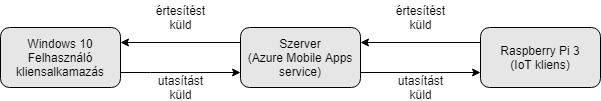
\includegraphics[width=\linewidth]{images/application_diagram.jpg}
    \caption{Az alkalmazás struktúrája}
    \label{fig: Az alkalmazás struktúrája}
\end{figure}

\chapter{Felhasználói dokumentáció}

\section{Minimális rendszerkövetelmények}
    A felhasználónak az alábbiakra van szüksége a program használatához:

    \begin{itemize}
        \item Egy Raspberry Pi 3 Model B mikroprocesszor, Windows 10 IoT Core operációs rendszerrel
        \item Windows 10 asztali vagy mobil eszköz
        \item Facebook profil
    \end{itemize}

\section{Raspberry Pi}

\subsection{Az eszközről}
    A Raspberry Pi egy bankkártya méretű, egyetlen áramköri lapra integrált számítógép, melyet az Egyesült Királyságban
    helyeztek forgalmomba 2012-ben, főleg oktatási célokra. Azóta számos változata megjelent, a szakdolgozat elkészítéséhez
    egy Raspberry Pi 3 Model B-t használtam. Számos bemenettel rendelkezik, többek között Ethernet csatlakozóval, HDMI, USB
    portokkal, a felhasznált modell pedig már beépített Wi-Fi adapterrel is. Többféle operációs rendszert telepíthetünk rá,
    köztük a Windows 10 IoT Core-t is, így kiválóan alkalmas arra, hogy futtathassuk rajta az IoT (Internet of Things) kliensalkalmazást.
    A továbbiakban a mikroprocesszor konfigurálása következik.

\begin{figure}[h!]
    \hspace{5cm}
    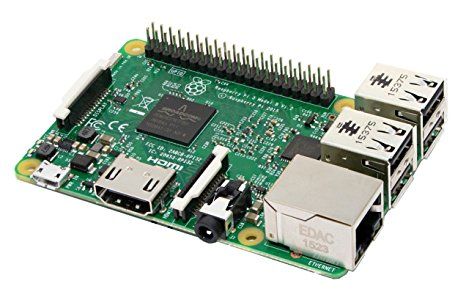
\includegraphics[width=6cm]{images/raspberry_pi3.jpg}
    \caption{Raspberry Pi 3 Model B}
    \label{fig: Raspberry Pi 3}
\end{figure}

\subsection{Beszerzés}
    A program futtatásához az eszköz korábbi verziói is megfelelőek lehetnek, azonban érdemes lehet a fent említett Raspberry Pi 3
    Model B -t, illetve az ennél újabb kiadásokat beszerezni, mivel ezek bizonyítottan elég erős hardverrel és csatlakozókkal rendelkeznek
    a feladat ellátásához. A szükséges komponensek:

\begin{itemize}
    \item Raspberry Pi 3 model B 1GB RAM Quad Core 2016-os alaplap
    \item 1.2A-es Sunny tápegység, 24 órás üzemre tervezve
    \item Legalább 8GB tárolókapacitású microSD kártya
\end{itemize}

    Az eszközt magyar viszonteladóktól is be lehet szerezni, valamint lehetőség van különböző előre összeállított csomagokat megvásárolni,
     melyek a fent említett kötelező elemeken túl tartalmazhatnak védőtokot az alaplapnak, illetve előtelepített operációs rendszert.

    A dolgozathoz használt kiszerelés az alábbi \href{https://malnapc.hu/yis/raspberry-pi-3-quad-core-suli-kit}{linken} elérhető.

\subsection{Operációs rendszer telepítése Raspberry Pi eszközre}

\subsubsection{Telepítés előtelepített SD kártyáról}
    Ha olyan verziót vásároltunk, melyhez előtepített operációs rendszert járt, akkor nincs más dolgunk, helyezzük be az SD kártyát
    az alaplapba, kössük össze a tápegységgel, helyezzük áram alá, s az eszköz azonnal elindul. Egy HDMI kábel segítségével kössük össze
    monitorunkkal, a vezérléshez szükség lesz legalább egy egérre. Az internetelérés történhet Ethernet csatlakozón, vagy (legalább Raspberry
    Pi 3 esetén) Wi-Fi-n keresztül is. Ha mindent jól csináltunk, akkor az eszköz rövid betöltés után megjelenít egy ablakot,
    melyben kiválaszthatjuk az általunk kívánt operációs rendszert. Többet is telepíthetünk, és javasolt is az alapértelmezett Raspbiant,
    valamint számunkra létfontosságú Windows 10 IoT Core-t. Ezt a Raspberry le fogja tölteni, ezért \textbf{elengedhetetlen} az internetkapcsolat.
    Az eszköz automatikusan telepíti a kiválasztott rendszereket, miután végzett, a mikroprocesszorunk használatra alkalmas.

\begin{figure}[h!]
    \hspace{5cm}
    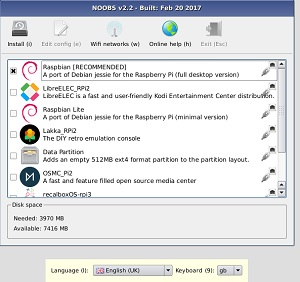
\includegraphics[width=6cm]{images/rpi_os_setup.jpg}
    \caption{Raspberry Pi Operációs rendszer kiválasztása}
    \label{fig: Raspberry Pi Operációs rendszer}
\end{figure}

\subsubsection{Telepítés nem előtelepített SD kártyáról}
    Ha nincs előre telepítve a szükséges operációs rendszer, akkor nekünk kell letölteni hivatalos forrásból.
    Ehhez a microsoft készített egy könnyen kezelhető felületet, a Windows 10 IoT Core Dashboardot, melyet
    \href{https://developer.microsoft.com/en-us/windows/iot/Downloads.htm}{ide} kattintva tudunk letölteni.
    Telepítsük fel az alkalmazást, majd kattintsunk a "\textbf{Set up a new device}" fülre, töltsük ki a szükséges adatokat, helyezzük
    az SD kártyát a számítógépünkbe. A "\textbf{Download and install}" lehetőségre klikkelve az alkalmazás telepíti nekünk
    az operációs rendszert.
    Ezt követően a lépések megegyeznek az előtelepítéses utasításokkal, tegyük a microSD-t a mikroprocesszorunkba, csatlakoztassuk
    a tápegységet, szükséges perifériákat, a rendszer rövid időn belül betölt.

    A részletes leírás az alábbi linken tekinthető meg: \url{https://www.windowscentral.com/how-install-windows-10-iot-raspberry-pi-3}

\subsection{Lámpa csatlakoztatása Raspberry Pi eszközhöz}
    Mivel nem rendelkezem mérnöki háttérismeretekkel, ezért nem egy valódi lámpát, hanem egy LED-et használtam a szakdolgozatom
    elkészítése során, így a LED működtetéséhez szükséges lépéseket, eszközöket fogom ismertetni.

\subsubsection{Szükséges elemek}

\begin{enumerate}
    \item \textbf{Egy} tetszőleges színű LED 2 - 2.5V-os fényforrás
    \item \textbf{Egy} próbapanel
    \item \textbf{Egy} legalább 270 Ohm-os ellenállás, a szakdolgozathoz 470 Ohm-ost használtam
    \item \textbf{Két} darab ANYA-APA Jumper kábel
\end{enumerate}

\begin{figure}[h!]
    \centering
    \begin{subfigure}[b]{0.4\linewidth}
        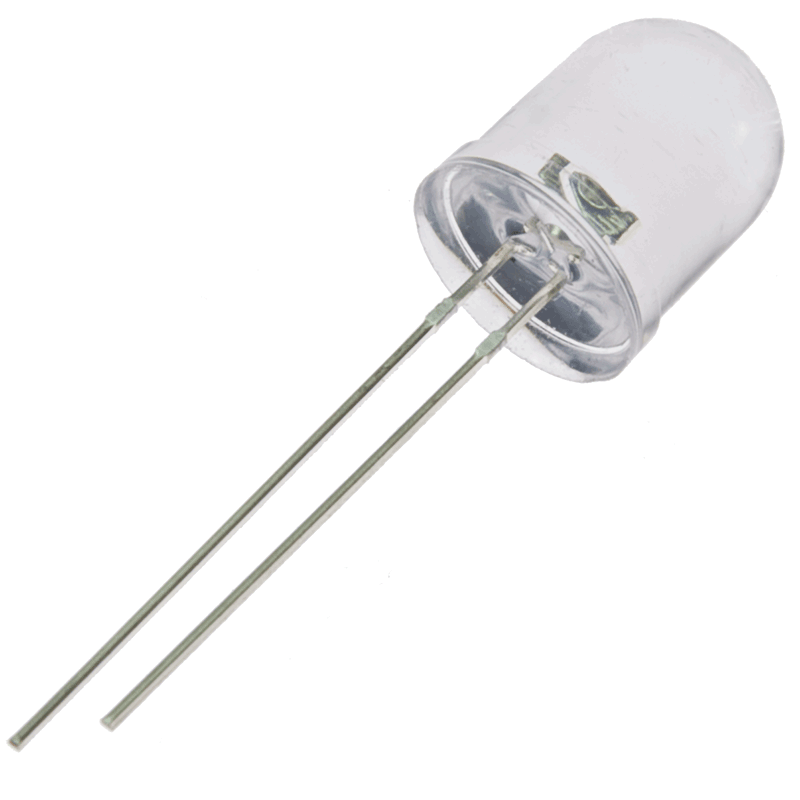
\includegraphics[width=\linewidth]{images/led.png}
        \caption{LED}
    \end{subfigure}
    \begin{subfigure}[b]{0.4\linewidth}
        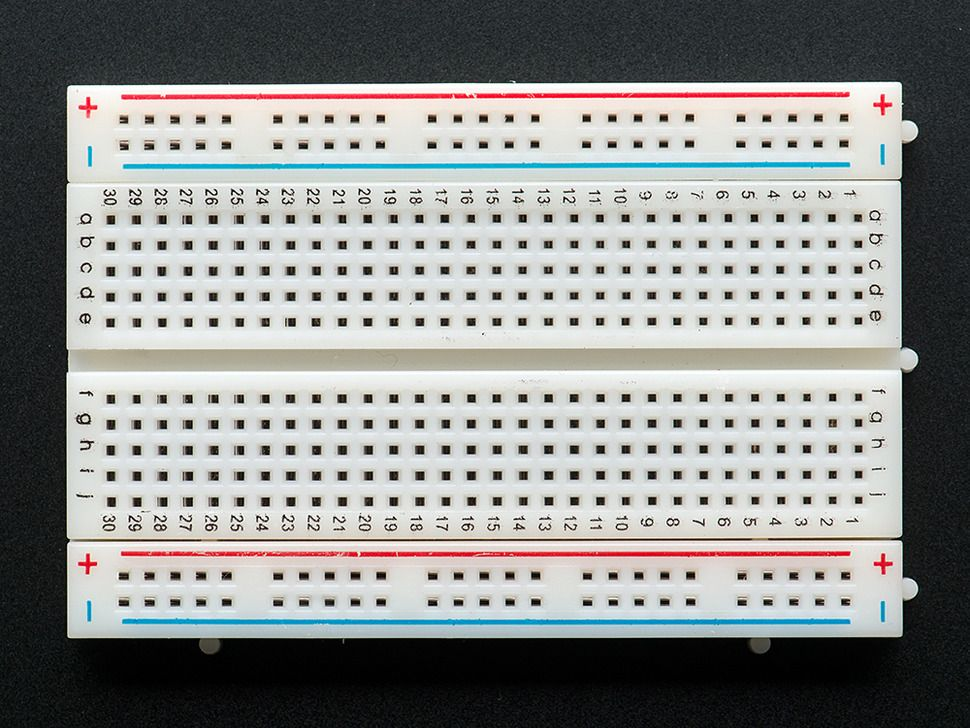
\includegraphics[width=\linewidth]{images/probapanel.jpg}
        \caption{Próbapanel}
    \end{subfigure}
    \begin{subfigure}[b]{0.4\linewidth}
        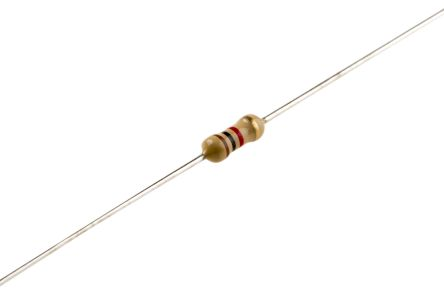
\includegraphics[width=\linewidth]{images/ellenallas.jpg}
        \caption{Ellenállás}
    \end{subfigure}
    \begin{subfigure}[b]{0.4\linewidth}
        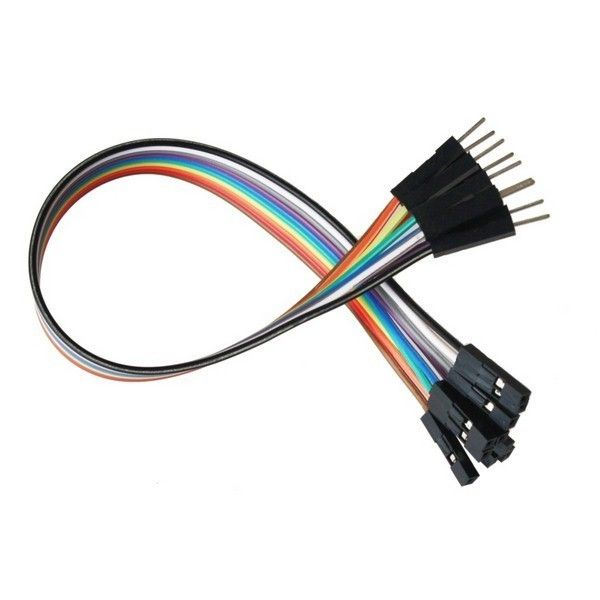
\includegraphics[width=\linewidth]{images/anyaapa.jpg}
        \caption{ANYA-APA kábel}
    \end{subfigure}
    \caption{Szükséges elemek}
    \label{fig:lampaelemek}
\end{figure}

\subsubsection{Összeszerelés}
    Miután beszereztük a szükséges elemeket, megkezdhetjük az összeszerelést. A próbapanelbe fogjuk belehelyezni a LED-et,
    az ellenállást, és a jumper kábel megfelelő végét. A másik végét a Raspberry Pi megfelelő GPIO pinjeire fogjuk csatlakoztatni.
    Ahhoz hogy a pinek között tudjunk tájékozódni, érdemes vásárolni egy kártyát, melyet rá lehet szúrni a tüskékre, és lehet látni
    a számozást.

\begin{figure}[h!]
    \hspace{5cm}
    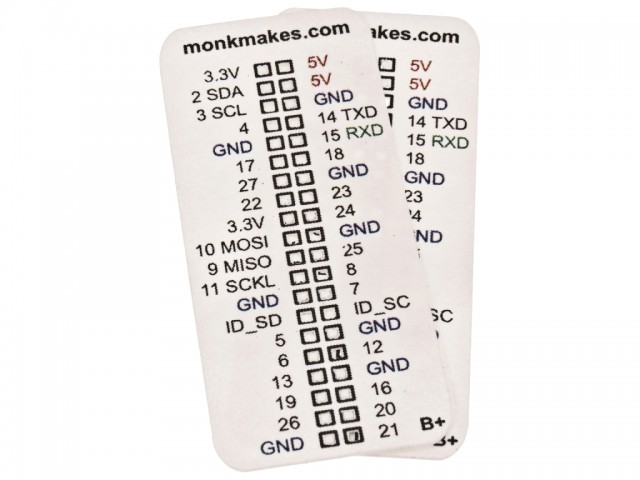
\includegraphics[width=6cm]{images/gpiohelper.jpg}
    \caption{A GPIO pinekhez kapható segítség}
    \label{fig: Pin segítség}
\end{figure}

    Készítsük magunk elé a mikroprocesszort és a többi szükséges eszközt, majd kövessük a következő lépéseket:

\begin{enumerate}
    \item A LED \textbf{hosszabbik} lábát szúrjuk bele a próbapanel \textbf{E} oszlopának \textbf{6.} sorába
    \item A LED \textbf{rövidebb} lába kerüljön egyel a hosszabbik alá, tehát a \textbf{E} oszlop \textbf{7.} sorába
    \item Hajlítsuk meg az ellenállás lábait úgy, hogy egy \textbf{U} alakot formáljon
    \item Egyik lábát helyezzük a LED hosszabbik vége mellé, tehát a \textbf{D 7} mezőbe
    \item A másik végződést szúrjuk a \textbf{D 1} helyre
    \item Fogjunk két ANYA-APA kábelt, az egyik APA végét szúrjuk az \textbf{A 1}, a másikét az \textbf{A 7} helyre, a LED
    rövidebb lábával egy sorba.
    \item Az első kábel ANYA végét csatlakoztassuk a Raspberry Pi 3.3V-os kimenetelére. Ez a bal felső kimenet a mikroprocesszoron.
    \item Végezetül a második kábel szabad végét kössük a 4-es GPIO pin-re. Ehhez használjuk a kis kártyát ha nem vagyunk biztosak
    magunkban.
\end{enumerate}

\begin{figure}[h!]
    \centering
    \begin{subfigure}[b]{0.4\linewidth}
        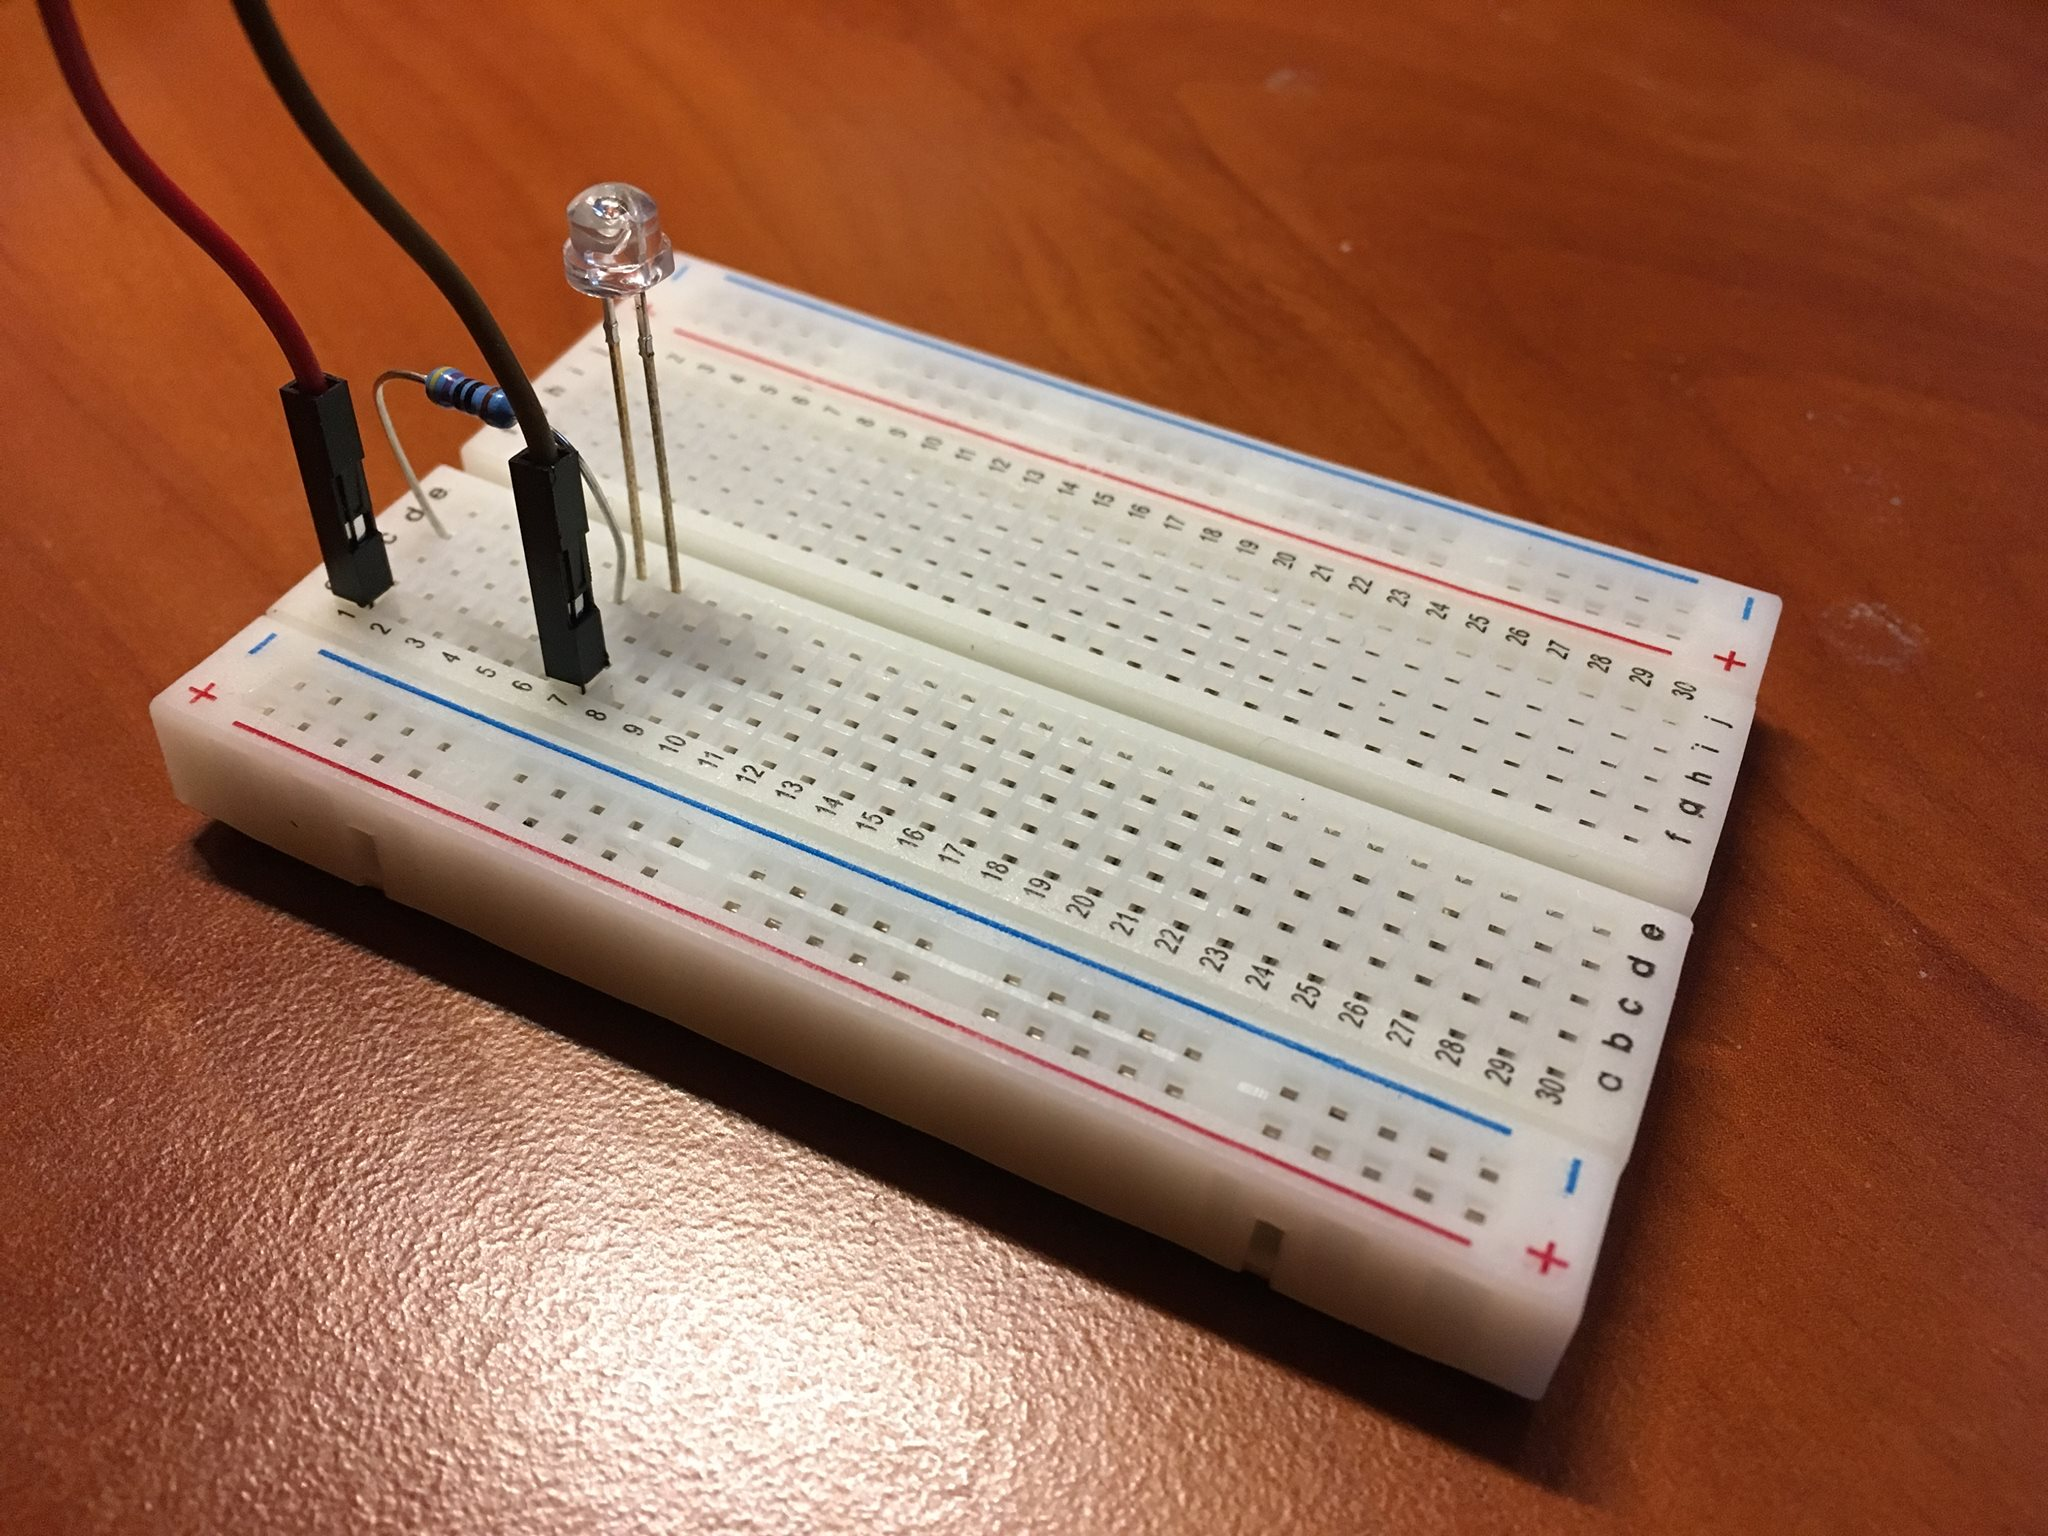
\includegraphics[width=\linewidth]{images/osszeszerelt1.jpg}
        \caption{Összeszerelt próbapanel oldalról}
    \end{subfigure}
    \begin{subfigure}[b]{0.4\linewidth}
        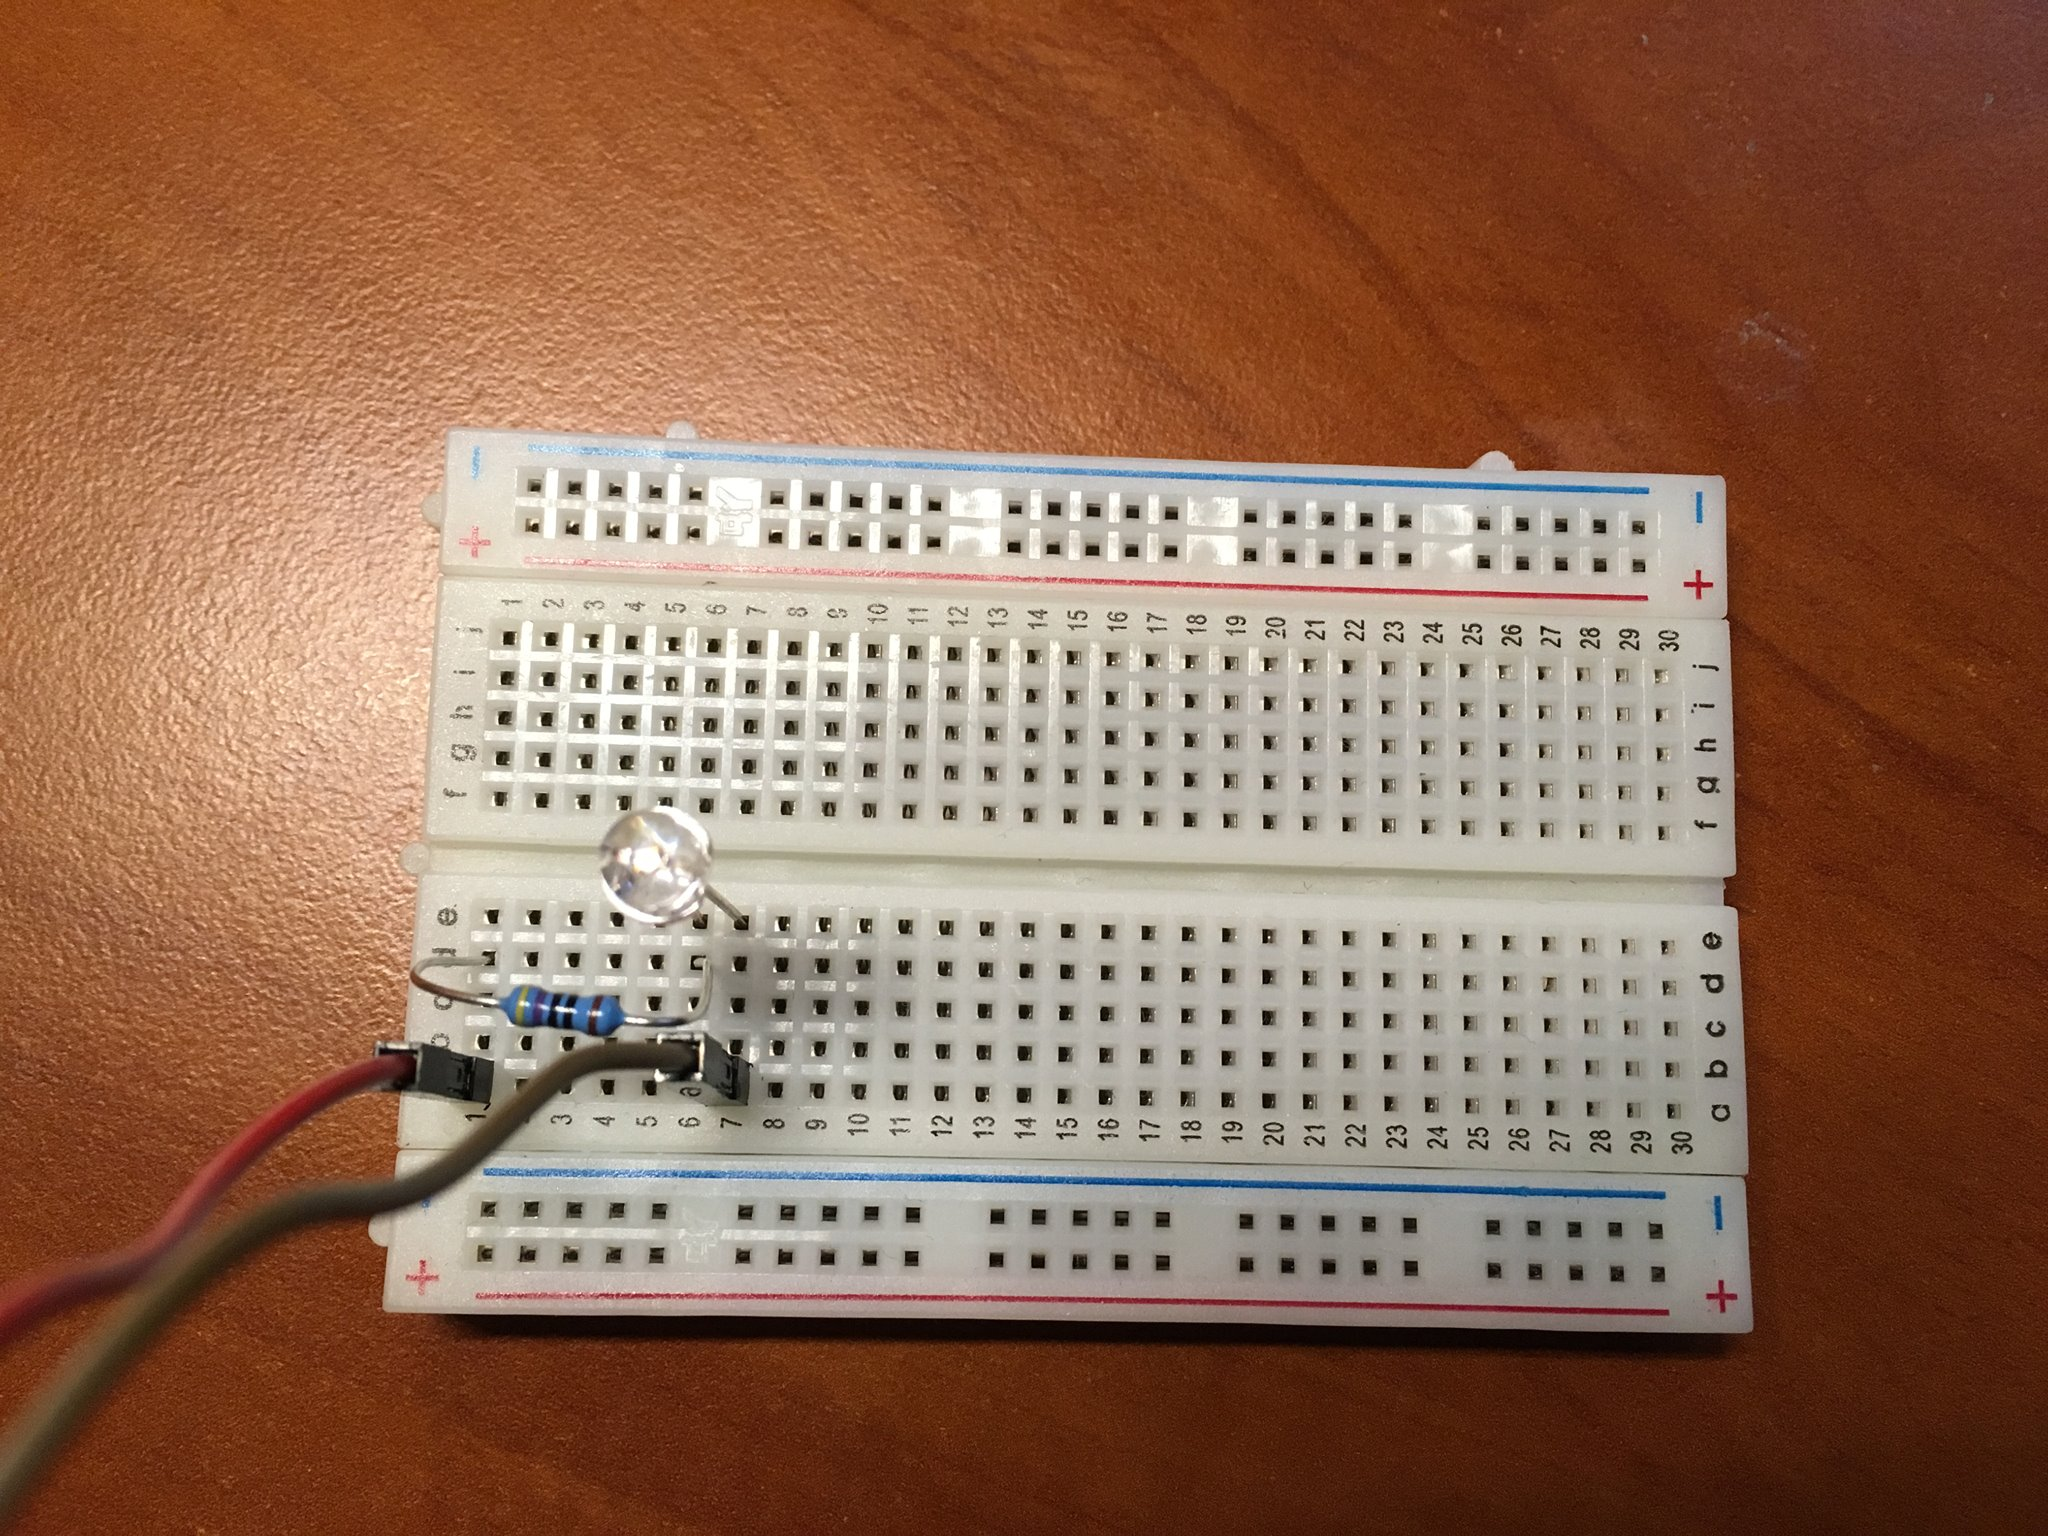
\includegraphics[width=\linewidth]{images/osszeszerelt2.jpg}
        \caption{Összeszerelt próbapanel felülről}
    \end{subfigure}
    \begin{subfigure}[b]{0.5\linewidth}
        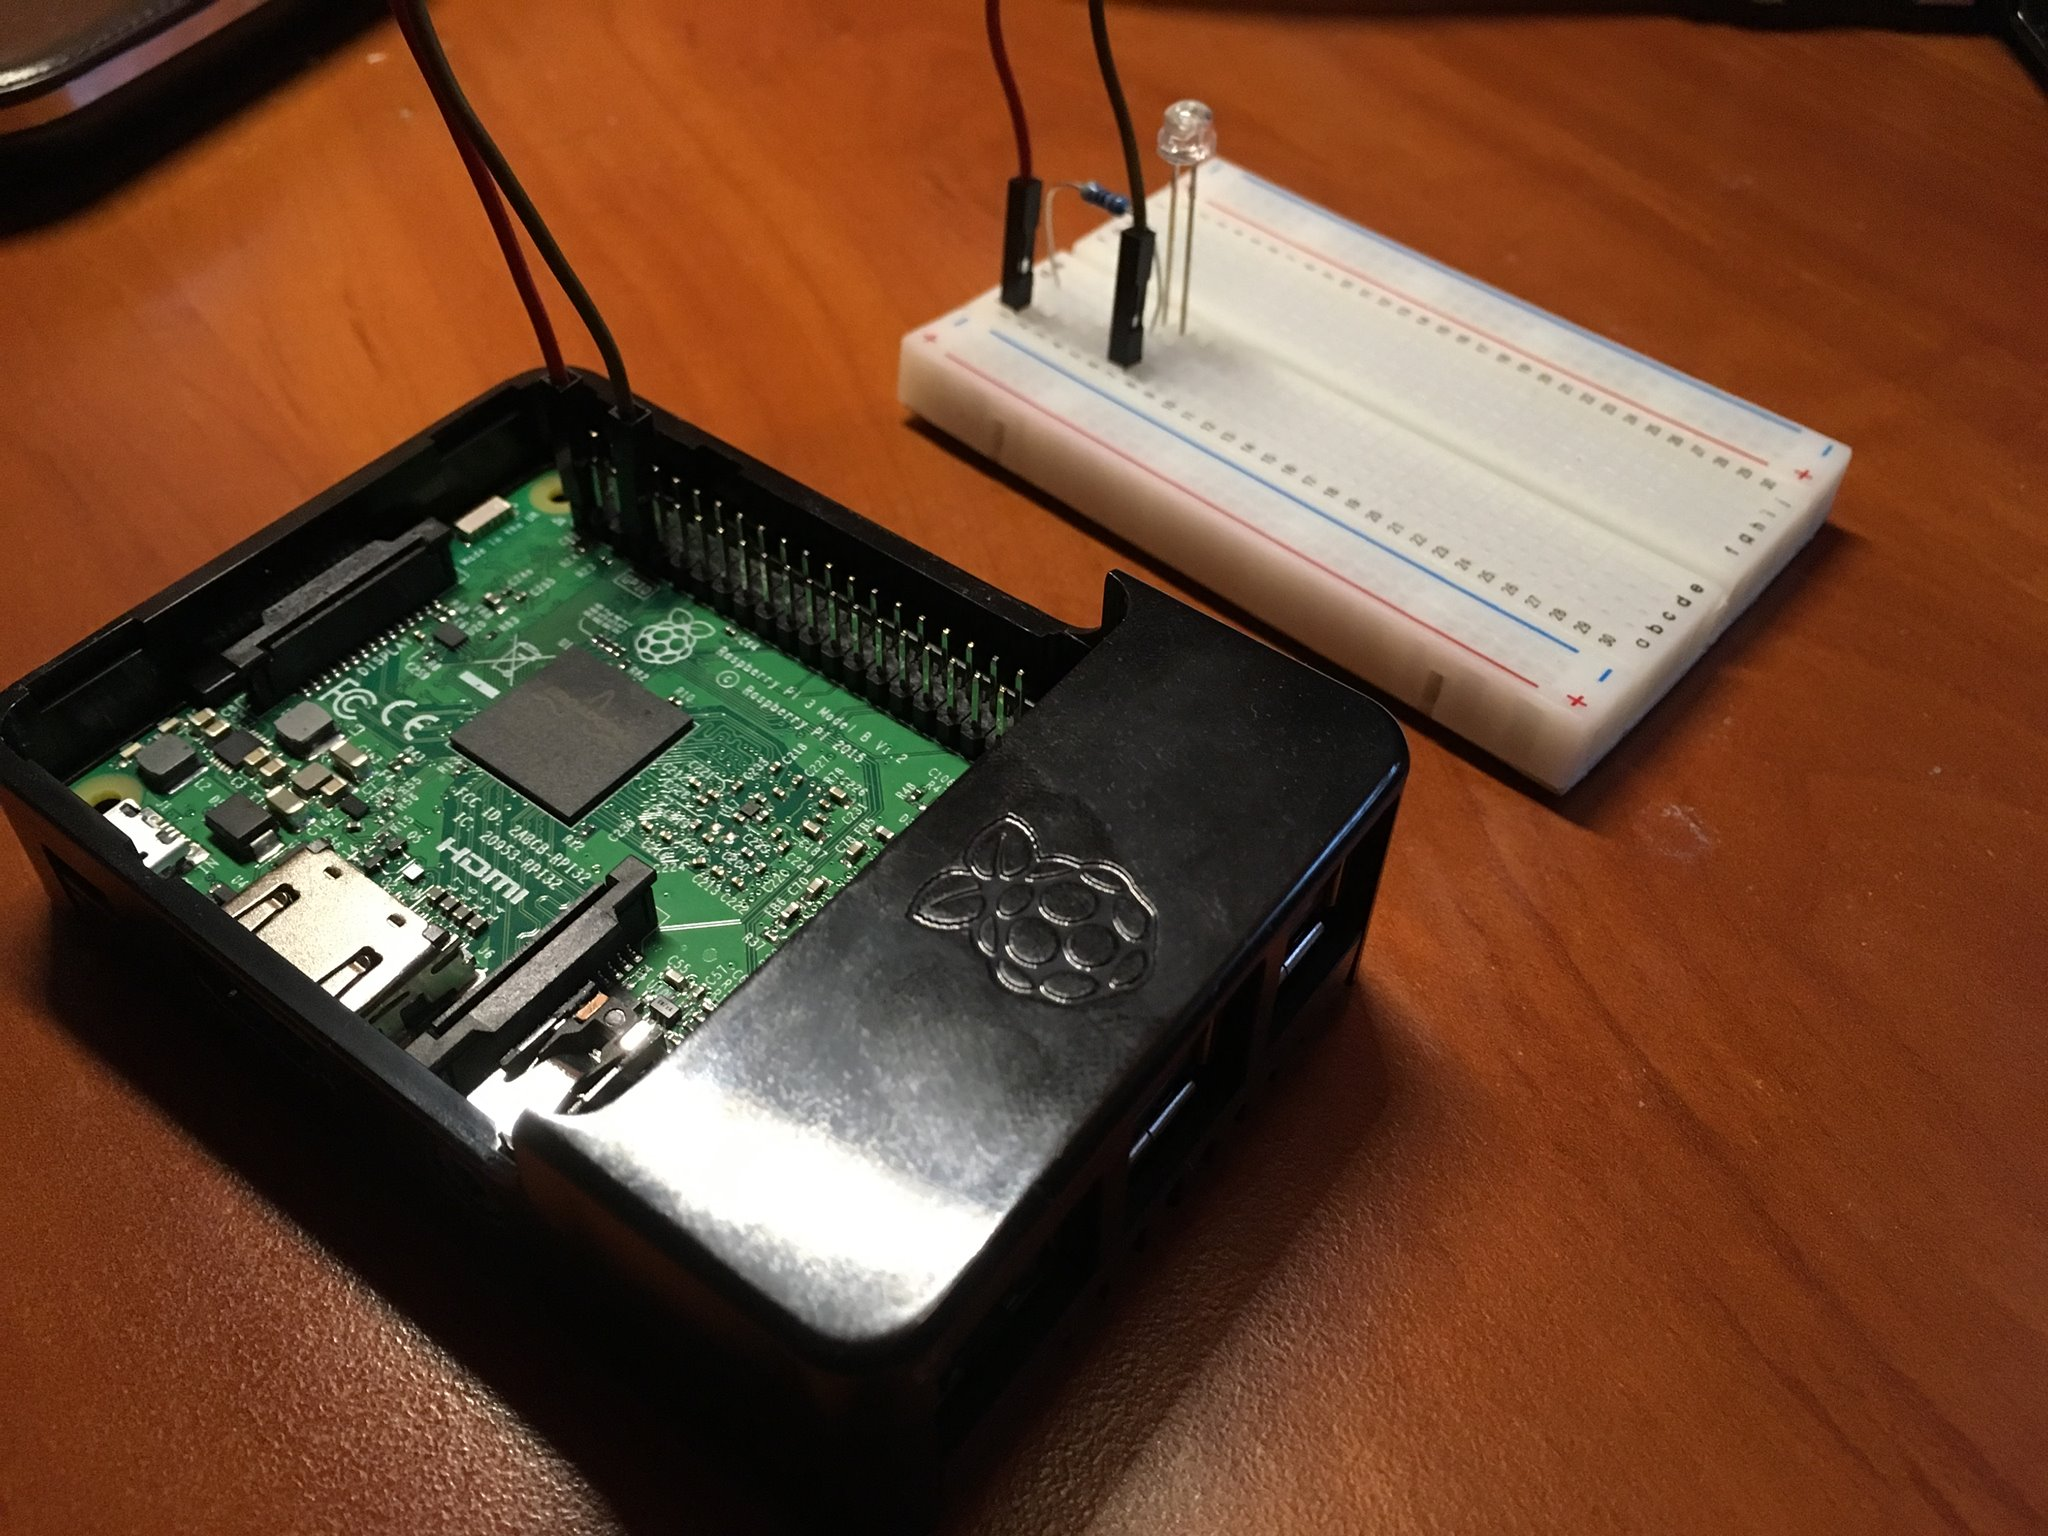
\includegraphics[width=\linewidth]{images/osszeszerelt3.jpg}
        \caption{Próbapanel rácsatlakoztatva a Raspberry Pi-re}
    \end{subfigure}
    \caption{Ha mindent jól csináltunk, a végeredmény így fog kinézni}
    \label{fig:összeszerelés}
\end{figure}

    A mikroprocesszorunk elkészült, most már alkalmas arra, hogy a IoT kliensalkalmazást futtassa.

\section{Telepítés}

\subsection{Asztali és mobilos környezetre}
    A felhasználói kliensalkalmazást a piactérről tudjuk letölteni, ha rákeresünk a ``KeepSwitched'' kulcsszóra. További
    teendőnk nincs, az érkező frissítéseket a program automatikusan letölteni és telepíti.
    A használathoz szükségünk van internet kapcsolatra és Facebook profilra.

\subsection{Raspberry Pi-re}
    Miután megfelelően összeszereltük a mikroprocesszorunkat, futtathatjuk az IoT kliensalkalmazást, melyet szintén a piactérről
    KeepSwitchedIoT néven tölthetünk le.
    Most következik az Application Deployment, tehát a letöltött alkalmazást futtatni fogjuk Raspberry Pi eszközünkön. Ezt
    megtehetjük böngészőből is, csak az Raspberry IP címére van szükségünk, amit leolvashatunk a képernyőről miután betöltött
    az eszköz.

\begin{figure}[h!]
    \hspace{5cm}
    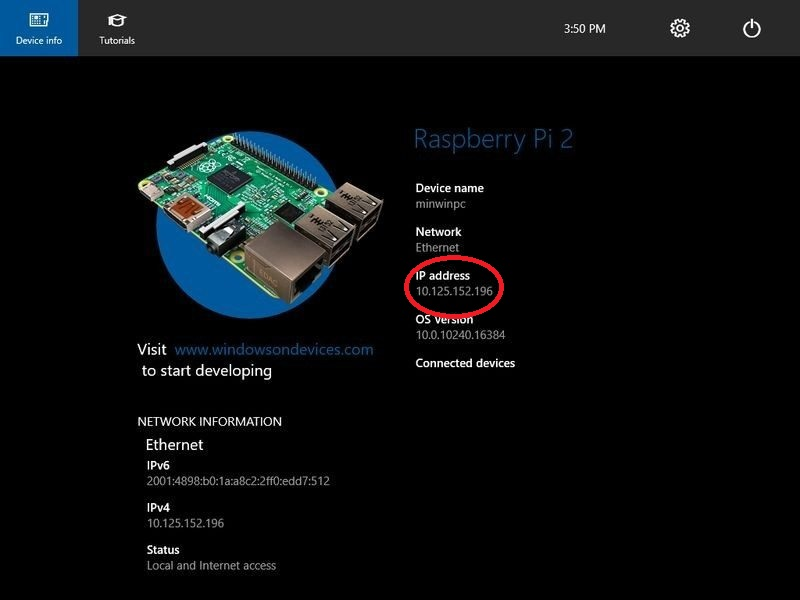
\includegraphics[width=6cm]{images/rpiip.jpg}
    \caption{A pirossal bekarikázott IP címre van szükségünk}
    \label{fig: Raspberry IP}
\end{figure}

    Másoljuk a kapott értéket a böngésző címsorába, és a \textbf{8080} - as porton keresztül tudjuk elérni eszközünket.
    Tehát ha az eszközünk IP címe például \textbf{192.168.0.105}, akkor az alábbi kerül a címsorba:

\begin{figure}[h!]
    \hspace{5cm}
    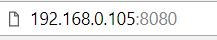
\includegraphics[width=6cm]{images/browserrpi.jpg}
    \caption{A címsorba írandó IP cím}
    \label{fig: Raspberry IP Browser}
\end{figure}

    Ha helyen másoltuk ki az IP címet, akkor a böngésző kérni fog tőlünk egy felhasználónevet és jelszót. A Windows 10 IoT Core
    operációs rendszer esetén az alapértelmezett adatok az alábbiak:

\begin{itemize}
    \item Felhasználónév: ``\textbf{Administrator}''
    \item Jelszó: ``\textbf{p@ssw0rd}''
\end{itemize}

    Ha sikeres volt az authentikáció, akkor a Windows Device Portal felülete fog megjelenni előttünk, mely így fest:

\begin{figure}[h!]
    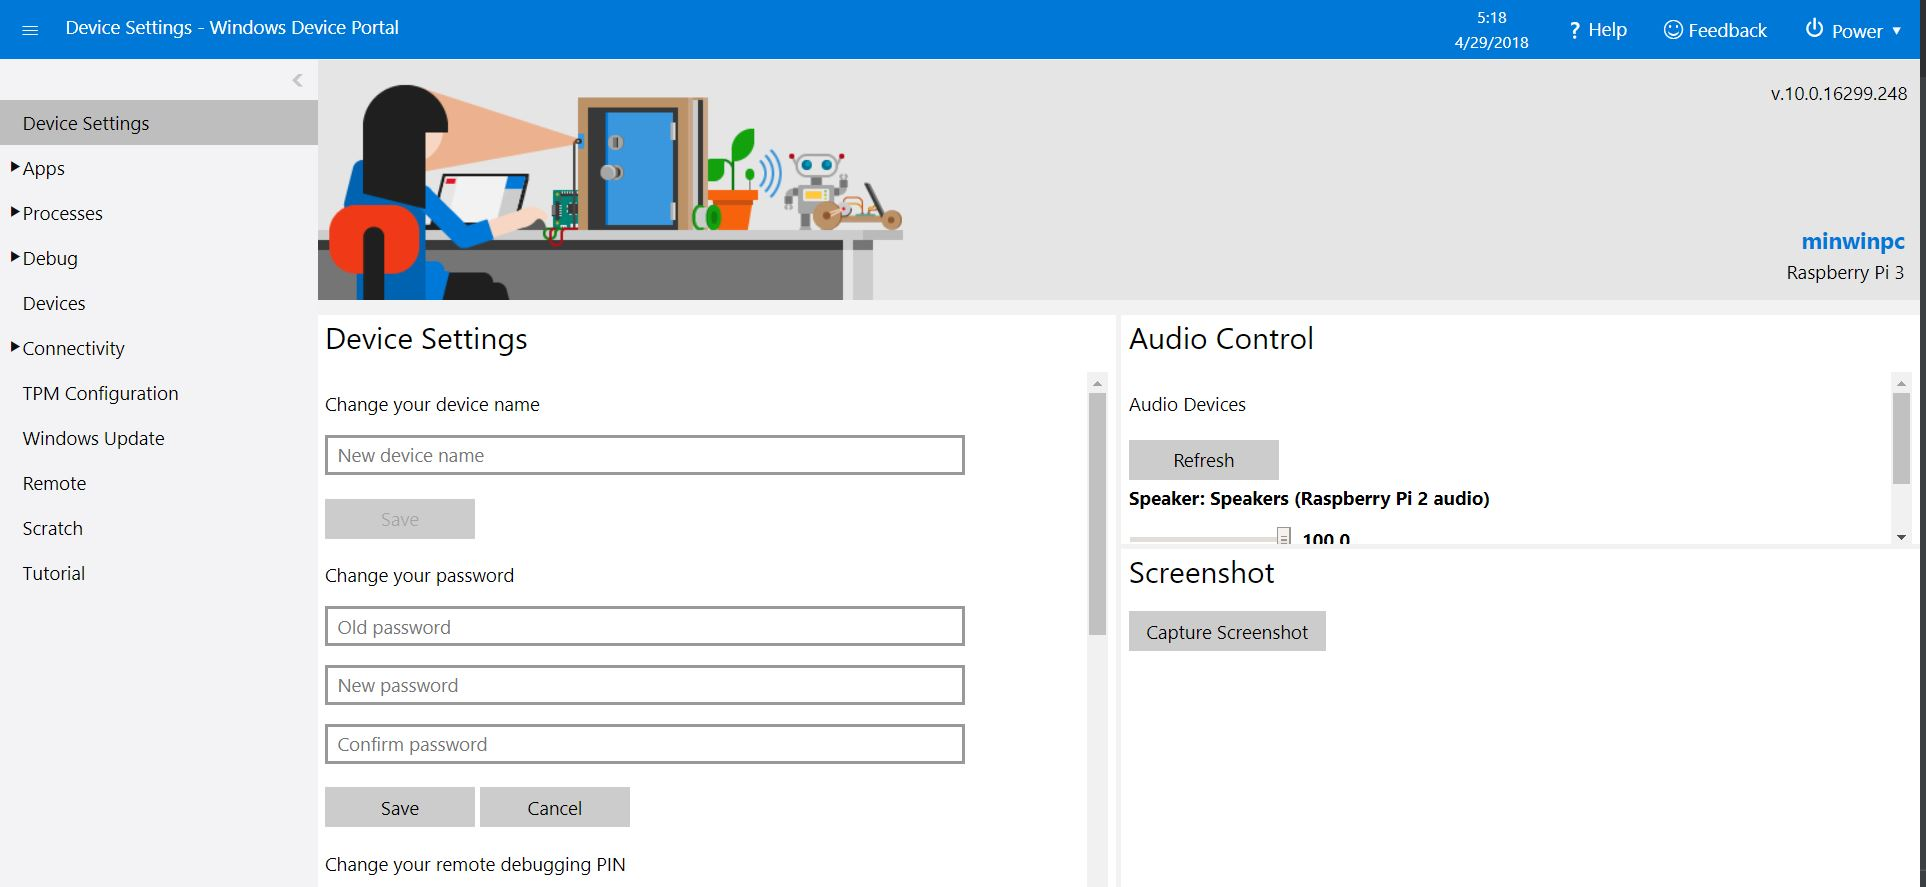
\includegraphics[width=\linewidth]{images/deviceportal.jpg}
    \caption{Windows Device Portal felülete}
    \label{fig: Windows Device Portal}
\end{figure}

    Ez egy nagyon hasznos felület, megváltoztathatjuk eszközünk nevét, jelszavát, felügyelhetjük a futó alkalmazásokat,
    kikapcsolhatjuk a Raspberry-t. De most egyelőre csak alkalmazást szeretnénk futtatni a mikroprocesszoron, így kattintsunk
    a bal oldalon található ``\textbf{Apps}"" fülre, majd az ``\textbf{Apps manager}"" lehetőségre.

\begin{figure}[h!]
    \centering
    \begin{subfigure}[b]{0.4\linewidth}
        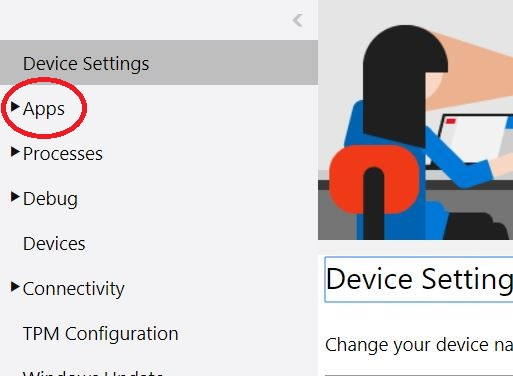
\includegraphics[width=\linewidth]{images/apps.jpg}
        \caption{Kattintsunk az Apps fülre}
    \end{subfigure}
    \begin{subfigure}[b]{0.4\linewidth}
        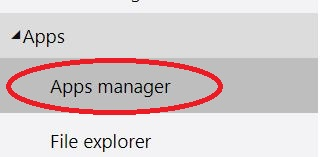
\includegraphics[width=\linewidth]{images/appsmanager.jpg}
        \caption{Majd az Apps Managerre}
    \end{subfigure}
    \caption{Navigáció alkalmazás hozzáadásához}
    \label{fig:Apps manager}
\end{figure}

    Most már majdnem készen vagyunk, válasszuk ki az ``\textbf{Add}'' lehetőséget, majd a megjelenő kis ablakban húzzuk bele
    a letöltött alkalmazást, vagy ki is kereshetjük a fájl böngészőből.

\begin{figure}[H]
    \centering
    \begin{subfigure}[b]{0.4\linewidth}
        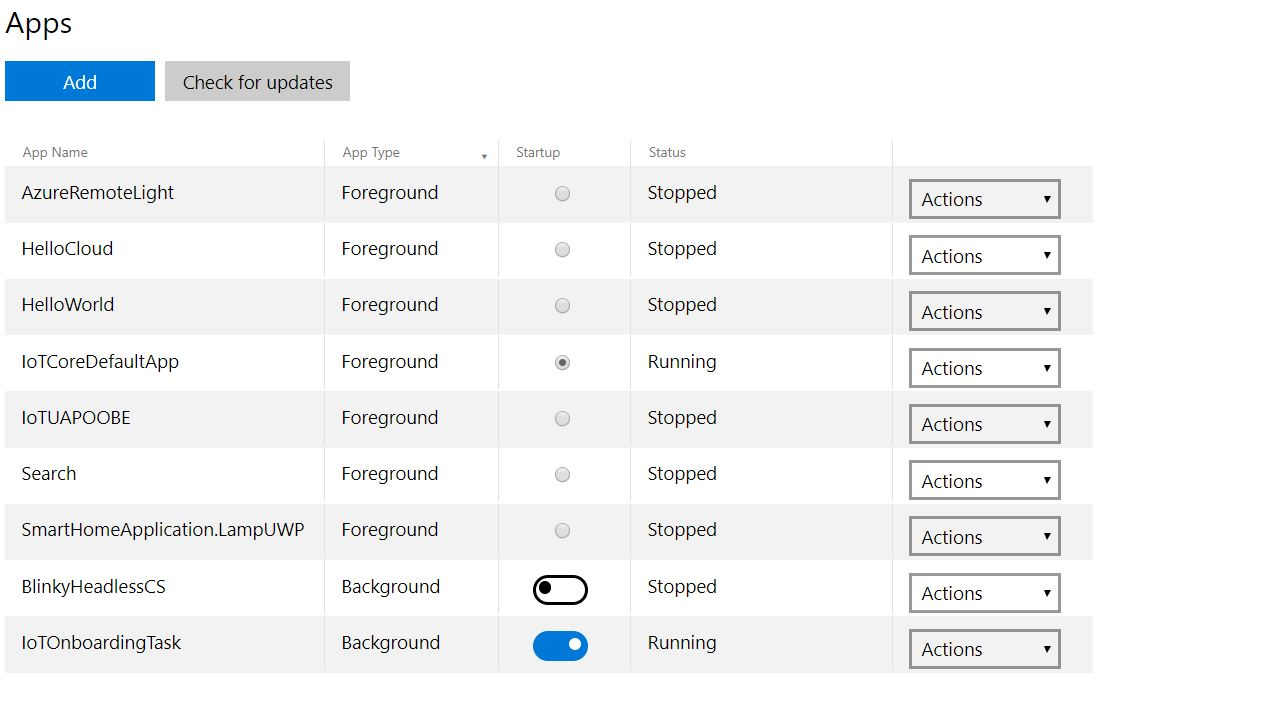
\includegraphics[width=\linewidth]{images/addapps.jpg}
        \caption{Kattinsunk az Add-ra}
    \end{subfigure}
    \begin{subfigure}[b]{0.4\linewidth}
        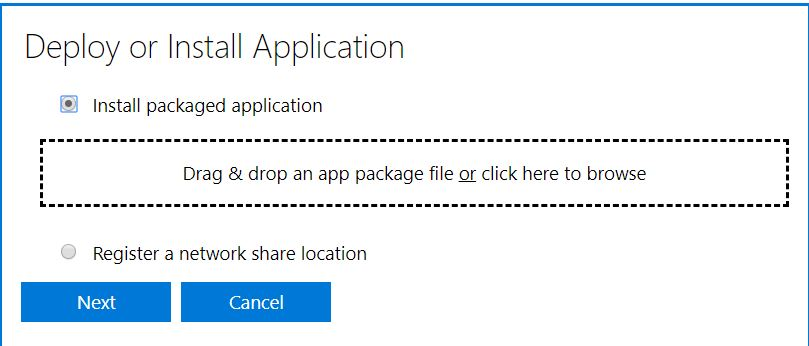
\includegraphics[width=\linewidth]{images/deploy.jpg}
        \caption{Húzzuk be, vagy keressük ki a letöltött alkalmazást}
    \end{subfigure}
    \caption{Alkalmazás hozzáadása}
    \label{fig:AddApps}
\end{figure}

    Ha mindent jól csináltunk, akkor a listában megjelenik alkalmazásunk és a mellette található legördülő menüben a ``\textbf{Start}''
    lehetőséget választva elindul az applikáció.

    \textbf{Fontos!} Áramszünet esetén a mikroprocesszor nem indítja el magától a programot, ehhez a ``\textbf{Startup}'' oszlopban
    be kell pipálnunk a lehetőséget.

\begin{figure}[h!]
    \centering
    \begin{subfigure}[b]{0.4\linewidth}
        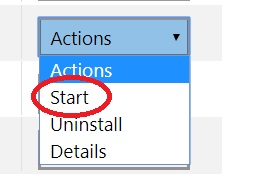
\includegraphics[width=\linewidth]{images/startapp.jpg}
        \caption{Indítsuk el az alkalmazást}
    \end{subfigure}
    \begin{subfigure}[b]{0.4\linewidth}
        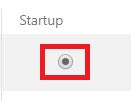
\includegraphics[width=\linewidth]{images/startupapp.jpg}
        \caption{Tegyük alapértelmezetté programunkat}
    \end{subfigure}
    \caption{Alkalmazás indítása és alapértelmezett futtatása}
    \label{fig:StartupApp}
\end{figure}

    A program telepítését befejeztük, az alkalmazás használatra kész!

\section{Felhasználói esetek}

\subsection{Bejelentkezés}
    A Windows 10 kliensalkalmazást csak bejelentkezett felhasználók tudják használni. Fontos, hogy \textbf{csak és kizárólag}
    Facebook profillal lehet belépni.

    A bejelentkezés lépései:

\begin{enumerate}
    \item Indítsuk el a programot, rövid idő után megjelenik a kezdőképernyő
    \item Kattintsunk a ``\textbf{Login with Facebook}'' feliratú kék hátterű gombra
    \item Ha van letöltött Facebook alkalmazásunk, akkor az, egyébként a böngésző fog elindulni
    \item Betöltődik a Facebook oldala, jelentkezzünk be email címünkkel, jelszavunkkal
    \item A Facebook engedélyt kér a profil használatára, engedélyezzük
    \item A program megjeleníti a lámpa hozzáadása nézetet, sikeresen bejelentkeztünk
\end{enumerate}

\subsection{Lámpa hozzáadása}
    A program célja, hogy távolról tudjunk vezérelni egy lámpát, ezért most végigmegyünk azokon a lépéseken, melyek a fényforrás
    hozzáadásához kellenek.

\begin{enumerate}
    \item Jelentkezzünk be a Windows 10 kliensalkalmazásba
    \item Sikeres bejelentkezés esetén a program a lámpa hozzadásáért felelős nézetre navigál, mely egy ``\textbf{GUID of Your lamp}''
    feliratból, egy szöveges beviteli mezőből, valamint egy egy gombból áll
    \item Ha még nem tettük volna meg, indítsuk el az IoT kliensalkalmazást, és olvassuk le a felhasználói felületén található
    5 karakterből álló egyéni azonosítót, a GUID-ot.
    \item Ezt a karaktersosorozatot másoljuk a szöveges beviteli mezőbe, majd kattintsunk az ``\textbf{Add lamp}'' feliratú gombra
    \item Ha megfelelő azonosítót adtunk be, akkor a lámpa sikeres felvételéről egy felugró ablak fog tájékoztatni minket
\end{enumerate}

\subsection{Lámpa vezérlése}
    Miután sikeresen csatlakoztattunk lámpát a profilunkhoz, szeretnénk vezérelni azt. Most az ehhez szükséges lépéseket tekintjük át.

\begin{enumerate}
    \item Jelentkezzünk be a Windows 10 kliensalkalmazásba
    \item Ha már sikeresen hozzáadtunk egy lámpát, akkor a képernyőn nem a szöveges beviteli mező lesz és a hozzáadás gomb, hanem
    egy felirat, mely tájékoztat arról, hogy már csatlakoztattunk eszközt
    \item Kattintsunk a bal felső sarokban lévő ``hamburgerger'' ikonra, ezzel előhozva a menüt
    \item Válasszuk a ``\textbf{Switch Lamp}'' menüpontot
    \item A megjelenített oldalon egy kapcsoló és egy gomb található. A kapcsolóval tudjuk a lámpát fel -és lekapcsolni, ``On''
    állapotban a fényforrás bekapcsolt, ``Off'' esetén pedig kikapcsolt állapotban van.
\end{enumerate}

    Most már sikeresen tudjunk vezérelni az alkalmazáson keresztül a profilunkhoz kapcsolt eszközt.

\subsection{Lámpa eltávolítása}
    Előfordulhat, hogy másik lámpát szeretnék vezérelni, így az előzőt el kell távolítani profilunkból. Ezt az alábbi pár lépésben
    megtehetjük.

\begin{enumerate}
    \item Jelentkezzünk be a Windows 10 kliensalkalmazásba
    \item Bal felül kattintsunk a ``hamburger'' ikonra, ezzel előhozva a menüt
    \item Válasszuk a ``\textbf{Switch Lamp}'' lehetőséget, megjelenik a vezérlő nézet
    \item Az oldal alján található egy ``\textbf{Delete Lamp}'' feliratú gomb egy kuka ikonnal. Erre kattintsunk
    \item A program egy felugró ablakon keresztül megkérdezi, hogy biztosan szeretnénk-e eltávolítani a csatolt eszközünket
    válasszuk a ``\textbf{Yes}'' opciót a törléshez
    \item Az alkalmazás visszaigazolja a sikeres műveletet
\end{enumerate}

\subsection{Statisztika megtekintése}
    Az alkalmazás lehetőséget ad arra, hogy megtekintsük lámpánk használati előzményeit, mikor történt fel -vagy lekapcsolás,
    és ekkor mennyi időre volt bekapcsolva a fényforrás, valamint összesen az áram alatt töltött napokat, órákat, perceket is
    számolja.

\begin{enumerate}
    \item Jelentkezzünk be a Windows 10 kliensalkalmazásba
    \item Bal felül kattintsunk a ``hamburger'' ikonra, ezzel megnyitva a menüt
    \item Kattintsunka ``\textbf{Statistic}'' menüpontra
    \item Az összesített időmennyiség az oldal tetején, a változtatások lisája az oldal alján található
\end{enumerate}

\subsection{Statisztika előzmények törlése}
    Megeshet, hogy már nem vagyunk kiváncsiak a lámpa előzményeire, ekkor lehetőségünk van törölni azokat. Ez például akkor
    fordulhat elő, ha égőt cseréltünk a fényforrásban, és szeretnénk lenullázni az időt, hogy nyomon tudjuk követni a friss
    égőt.

\begin{enumerate}
    \item Jelentkezzünk be a Windows 10 kliensalkalmazásba
    \item Bal felül kattintsunk a ``hamburger'' ikonra, ezzel megnyitva a menüt
    \item Válasszuk ``\textbf{Statistic}'' menüpontot
    \item Kattintsunk ``\textbf{Clear History}'' feliratú, kuka ikonnal rendelkező gombra
    \item A program megkérdezi hogy biztosan szeretnénk-e törölni az előzményekett, a ``\textbf{Yes}'' opcióval véglegesíthetjük
    a döntést
\end{enumerate}

    \textbf{Fontos!} A törlés végleges, az adatokat később semmilyen formában nem lehet visszanyerni, valamint az összes lámpára
    csatlakozott felhasználó számára kitörli az előzményeket.

\subsection{Kijelentkezés a programból}
    Lehetőség van kijelentkezvi a Windows 10 kliensalkalmazásból, hasznos lehet ha más felhasználóknek kell átadnunk az általunk
    használt mobilt vagy asztali számítógépet.

\begin{enumerate}
    \item Tegyük fel, hogy éppen a vezérlő nézeten állunk. A kijelentkezés ugyanúgy működik az összes oldalról
    \item Bal felül kattintsunk a ``hamburger'' ikonra, ezzel megnyitva a menüt
    \item A menü legalján található kis ajtó ikonnal ellátott ``\textbf{Log Out}'' feliratű gomb. Erre kattintsunk
    \item A program megkérdezi hogy biztosan szeretnénk-e kijelentkezni az alkalmazásból. A ``\textbf{Yes}'' gombra kattintva
    véglegesíthetjük a döntést
\end{enumerate}

\section{Felhasználói felület}

\subsection{IoT Kliensalkalmazás}
    A Raspberry Pi-n futó alkalmazás nem rendelkezik különösebb felhasználói felülettel, csupán egy szürke háttérből, és egy
    szövegdobozból áll. A szövegdobozban szerepel az eszköz GUID-ja, egyedi azonosítója, mely segítségével tudunk egy lámpát
    hozzáadni a profilunkhoz.

\begin{figure}[h!]
    \centering
    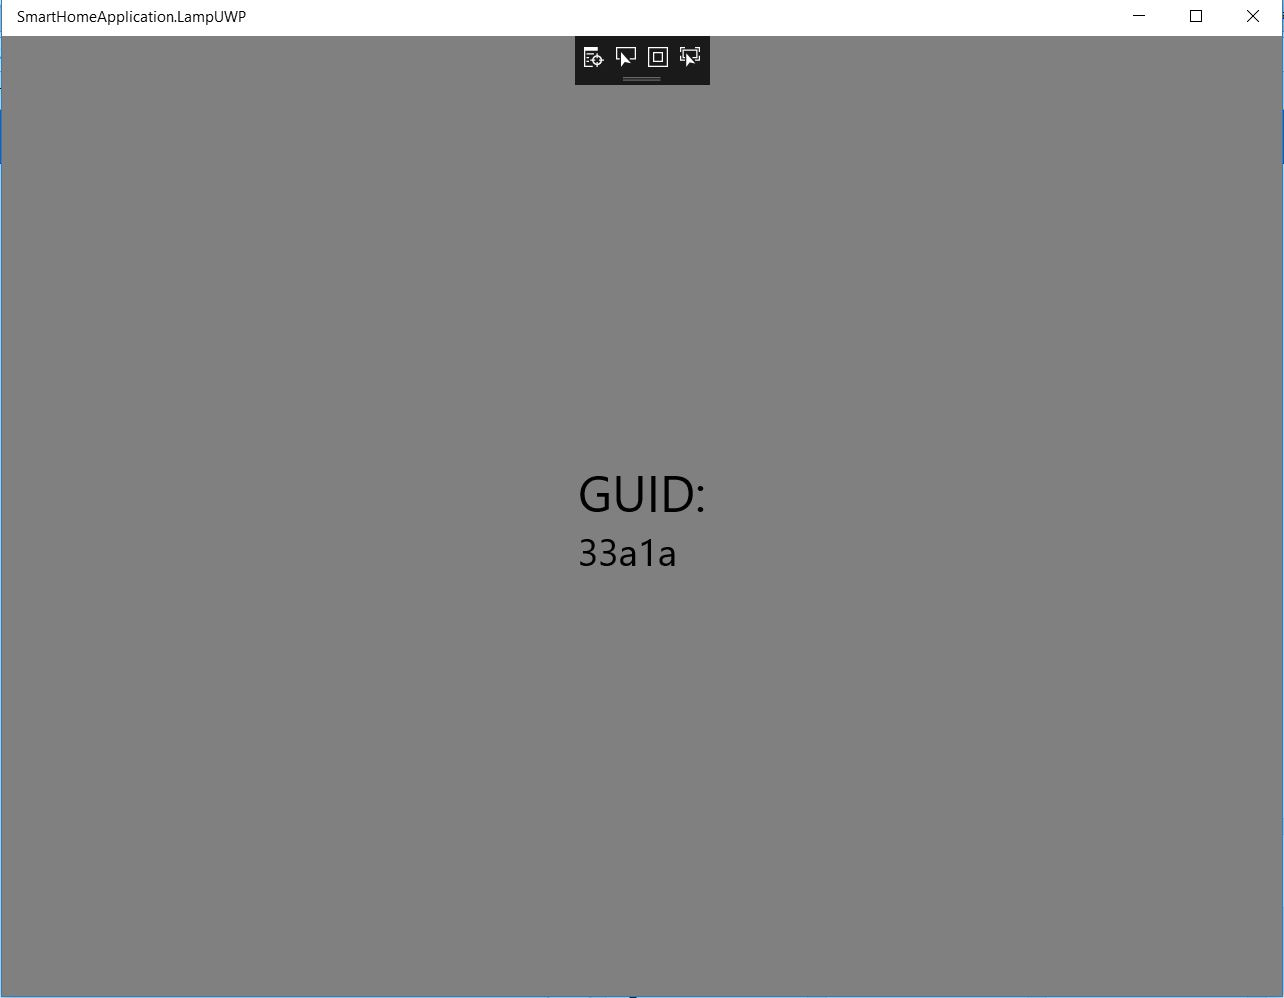
\includegraphics[width=6cm]{images/lampuwp.jpg}
    \caption{Az IoT kliensalkalmazás felülete}
    \label{fig: LampUWP}
\end{figure}

\subsection{Windows 10 kliensalkalmazás}

\subsubsection{Bejelentkezés}
    Az alkalmazás indítása után egy szürke hátterű ablak jelenik meg üdvözlőszöveggel, középen pedig a bejelentkezéshez szükséges
    gombbal. Erre kattintva tudunk Facebookon keresztül belépni a programba.

\begin{figure}[H]
    \centering
    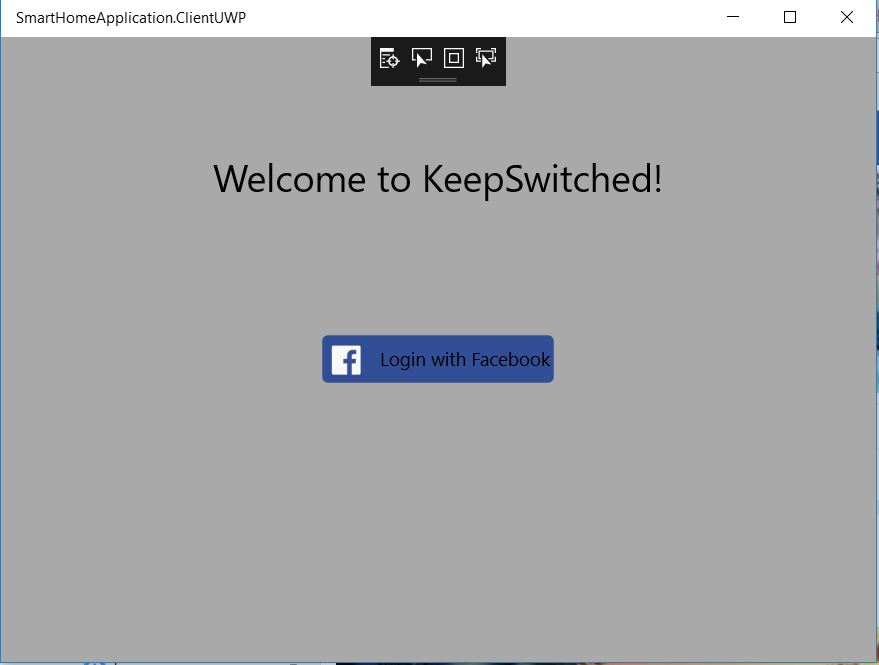
\includegraphics[width=6cm]{images/loginview.jpg}
    \caption{Bejelentkező ablak}
    \label{fig: Login}
\end{figure}

    \textbf{Fontos!} Az állandó internetkapcsolat alapkövetelmény, a program indításakor az alkalmazás ellenőrzi, hogy csatlakozunk-e
    a világhálóhoz, amennyiben nem, egy felugró ablak fog fogadni minket, mely tájékoztat a hibáról, majd bezárul a program.

\begin{figure}[H]
    \centering
    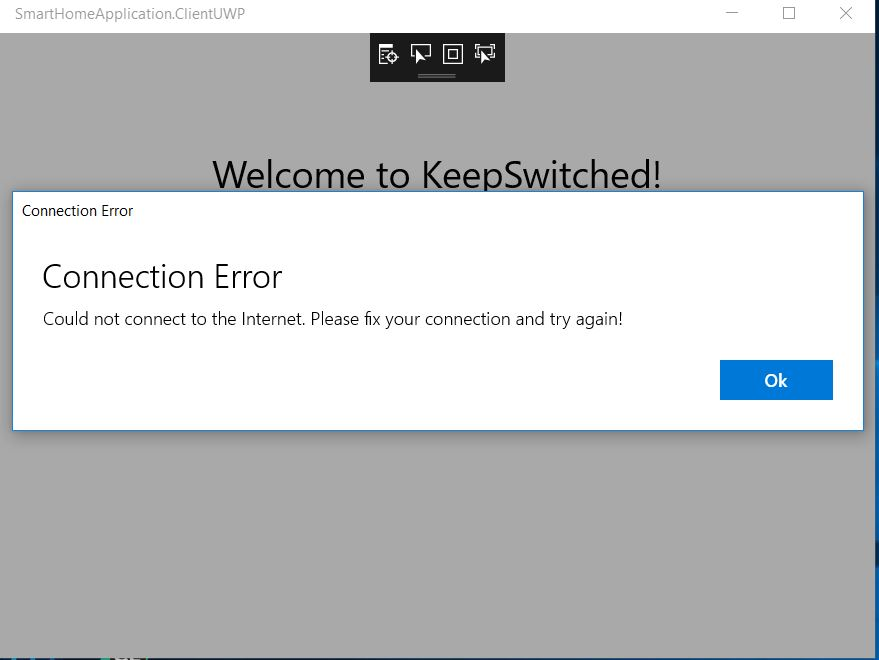
\includegraphics[width=6cm]{images/connectionerror.jpg}
    \caption{Internetkapcsolat hiánya esetén látható hibaüzenet}
    \label{fig: ConnectionError}
\end{figure}

\subsubsection{Menü}
    Bejelentkezés után a menüt a bal felső sarokban található ``hamburger'' ikonra kattintva tudjuk előhozni. Ez felel az
    alkalmazáson belüli navigációért, és itt van lehetőség kijelentkezésre is.

\begin{figure}[H]
    \centering
    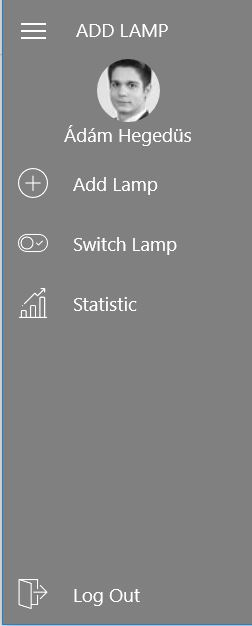
\includegraphics[width=3cm,height=6cm,keepaspectratio]{images/hamburgermenu.jpg}
    \caption{Hamburger menü}
    \label{fig: Hamburger}
\end{figure}

    A képen látható, hogy a ``hamburger'' ikon mellett található az éppen megnyitott lap neve, a minta esetében ``ADD LAMP'',
    alatta a Facebook profilképünk, és a nevünk.
    Továbbá a személyes adataink alatt találhatóak a nézetek, melyek közt navigálhatunk. Kezdetben a lámpa hozzáadásáért felelős
    oldal töltődik be, onnan válthatunk a menü segítségével. A választási lehetőség neve mellett egy kis ikon található, ez
    adhat egy kis segítséget abban, hogy az adott nézet miért felelős. A kijelentkezés gomb a menü alján található.

    Az alkalmazás az alábbi lehetőségeket kínálja:

\begin{itemize}
    \item ``\textbf{Add Lamp}'' Lámpa hozzadásáért felelős nézet. Ikonja egy plusz jel bekarikázva
    \item ``\textbf{Switch Lamp}'' A lámpa vezérléséért felelős nézet, továbbá itt tudjuk eltávolítani a profilunkhoz csatolt
    eszközt. Ikonja egy lámpakapcsoló
    \item ``\textbf{Statistic}'' A lámpa statisztikáit tudjuk ebben a nézetben szemügyre venni. Ikonja egy diagram melyen egy felfele
    mutató nyíl található
    \item  ``\textbf{Log Out}'' Ezen gomb segítségével tudunk kijelentkezni. Ikonja egy nyitott ajtó
\end{itemize}

\subsubsection{Lámpa hozzáadása nézet}
    Bejelentkezés után a program automatikan erre a nézetre irányít, vagy a menüben az ``\textbf{Add Lamp}'' lehetőségre
    kattintva juthatunk el ide.
    Amennyiben még nem rendelkezünk hozzáadott eszközzel, akkor egy szöveges beviteli mező és egy a nézet nevével megegyező
    feliratú gomb található az oldalon. Ha már csatlakoztattunk lámpát akkor az előbbi lehetőségek nem elérhetőek, helyette
    egy rövid szöveg fogad minket, miszerint már van fényforássunk, a többi oldal felkeresésével tudjuk vezérelni, statisztikáit
    megtekinteni.

\begin{figure}[h!]
    \centering
    \begin{subfigure}[b]{0.4\linewidth}
        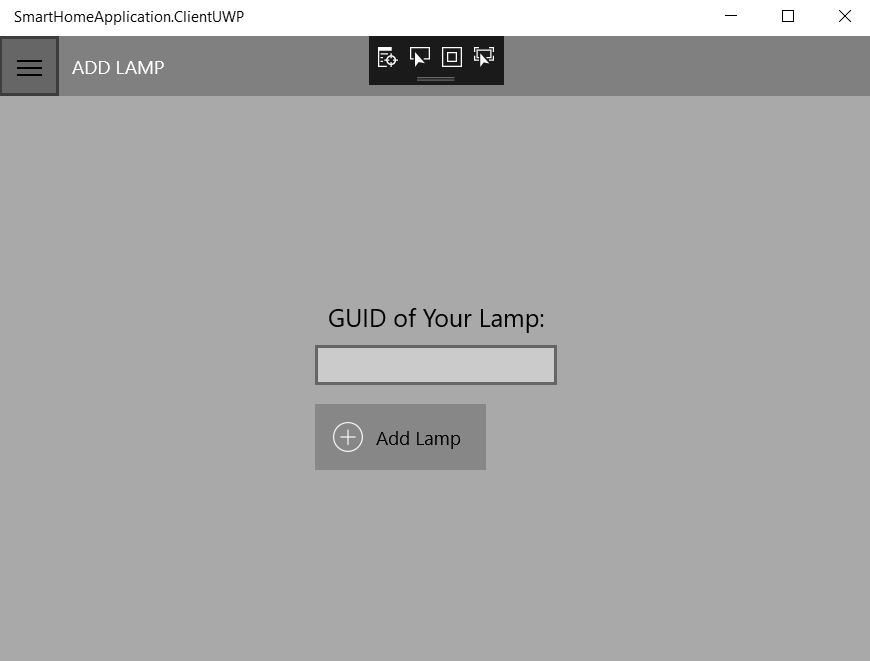
\includegraphics[width=\linewidth]{images/addlampview.jpg}
        \caption{Lámpa hozzadása nézet ha nincs még eszközünk}
    \end{subfigure}
    \begin{subfigure}[b]{0.4\linewidth}
        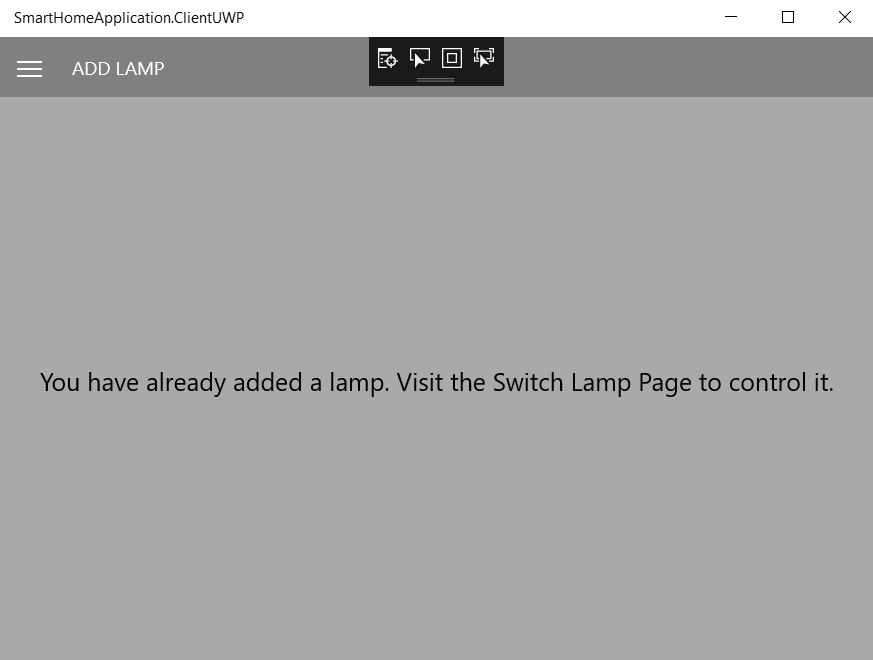
\includegraphics[width=\linewidth]{images/alreadyhaslamp.jpg}
        \caption{Lámpa hozzáadása nézet ha már van nézetünk}
    \end{subfigure}
    \caption{Lámpa hozzáadása nézet}
    \label{fig:AddLampView}
\end{figure}

    A lámpa hozzáadása az eszköz öt hosszúságú egyéni azonosítója segítségével történik, amennyiben nem megfelelő karaktersorozatot
    adunk be, a program hibaüzenetet dob.

\begin{figure}[H]
    \centering
    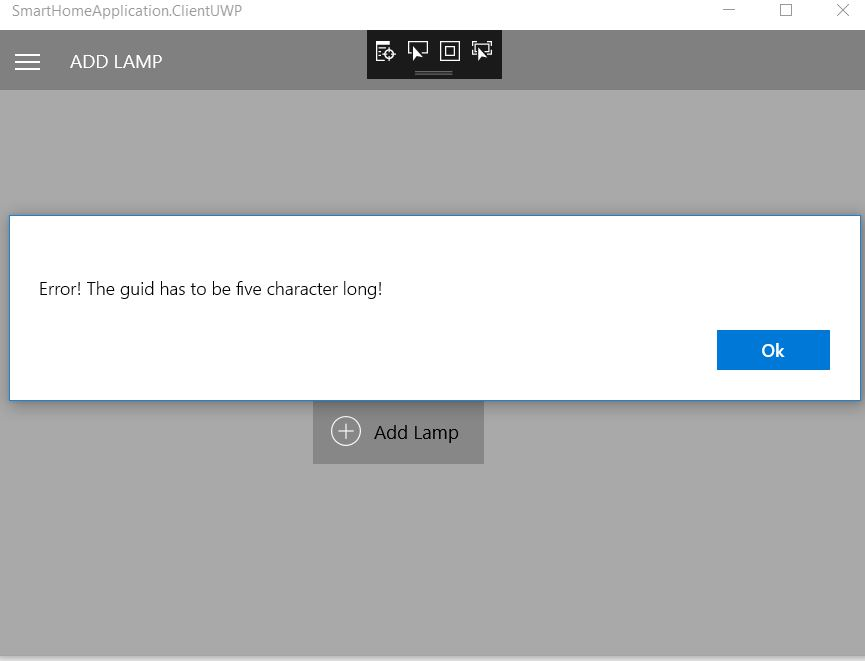
\includegraphics[width=6cm]{images/fivecharacter.jpg}
    \caption{Nem megfelelő hosszúságú GUID esetén kapott hibaüzenet}
    \label{fig: FiveCharacter}
\end{figure}

    Továbbá természetesen az is hibát szül, amennyiben nem létező GUID-ot írunk be, így a hozzáadás gombra kattintás után
    hibaüzenetet kapunk.

\begin{figure}[H]
    \centering
    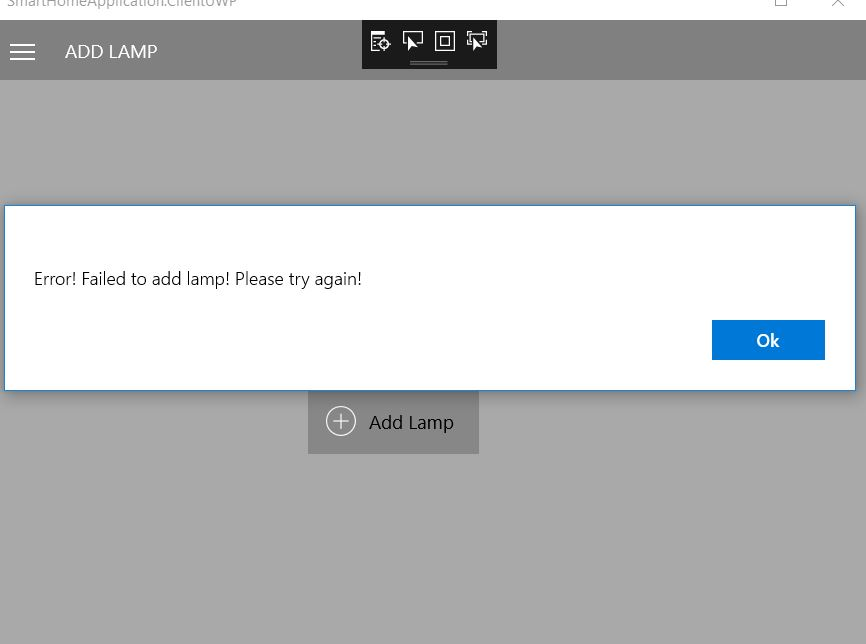
\includegraphics[width=6cm]{images/addfail.jpg}
    \caption{Nem létező GUID esetén hibaüzenetet kapunk}
    \label{fig: InvalidGuid}
\end{figure}

\subsubsection{Lámpa vezérlése nézet}
    Ez az oldal felelős a lámpa fel -és lekapcsolásáért, valamint itt tudjuk leválasztani az eszközt a profilunkról. Amennyiben
    nem rendelkezünk fényforrással, akkor nem jelenik meg a kapcsoló és a törlés gomb, az alkalmazás egy rövid üzenettel kér
    arra, hogy csatlakoztassunk egy lámpát, majd utána vezéreljük azt.

\begin{figure}[H]
    \centering
    \begin{subfigure}[b]{0.4\linewidth}
        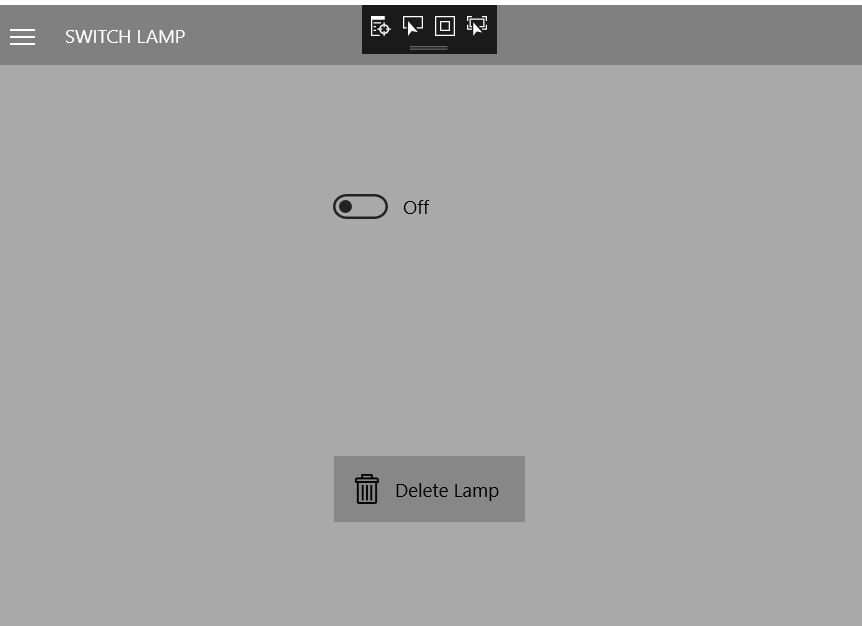
\includegraphics[width=\linewidth]{images/switchview.jpg}
        \caption{Lámpa vezérlése}
    \end{subfigure}
    \begin{subfigure}[b]{0.4\linewidth}
        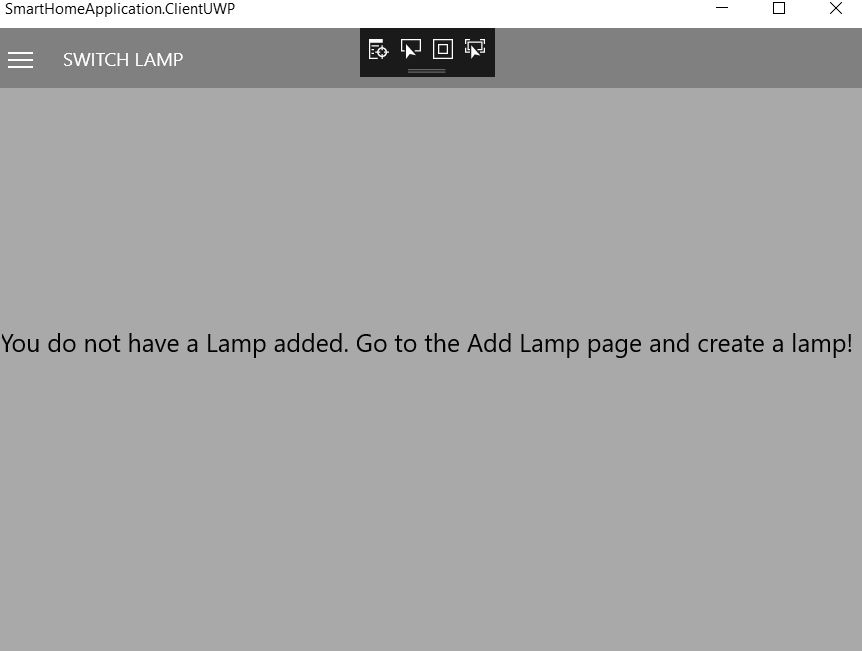
\includegraphics[width=\linewidth]{images/switchdonthavelamp.jpg}
        \caption{Lámpa vezérlése ha nincs lámpánk}
    \end{subfigure}
    \caption{Lámpa vezérlése nézet}
    \label{fig:SwitchLampView}
\end{figure}

    Ha úgy döntünk hogy eltávolítjuk a profilunkhoz kapcsolt lámpát, akkor kattintsunk a ``\textbf{Delete Lamp}'' feliratú
    gombra, a program megkérdezi hogy véglegesítjük-e a döntést. Ha igen, akkor a sikeres törlést követően értesítést kapunk
    a művelet befejeztéről.

\begin{figure}[H]
    \centering
    \begin{subfigure}[b]{0.4\linewidth}
        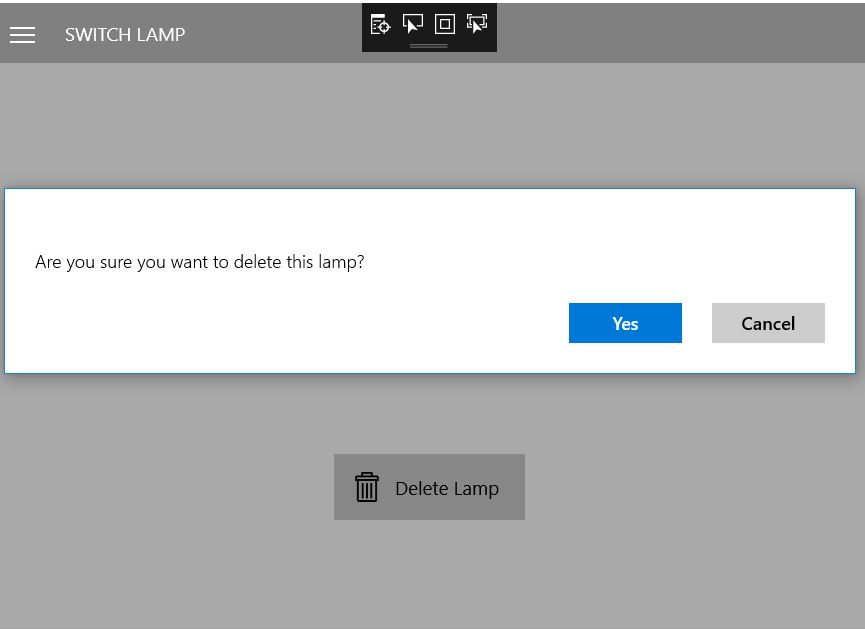
\includegraphics[width=\linewidth]{images/suredelete.jpg}
        \caption{Törlést megerősítő felugró ablak}
    \end{subfigure}
    \begin{subfigure}[b]{0.4\linewidth}
        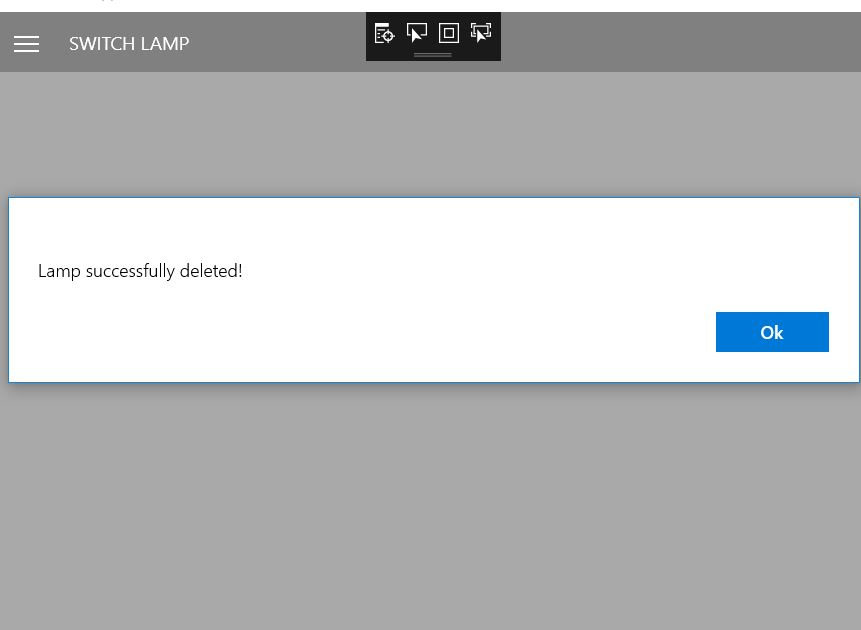
\includegraphics[width=\linewidth]{images/deletesuccess.jpg}
        \caption{Sikeres törlés értesítő üzenet}
    \end{subfigure}
    \caption{Lámpa törlése}
    \label{fig:LampDelete}
\end{figure}

    \textbf{Fontos!} A törlés ebben az esetben is végleges, nem lehet visszaállítani a korábbi állapotot, azonban ha szeretnénk,
    ugyanazt a lámpát az ``Add Lamp'' oldalon gond nélkül felvehetjük újra.

\subsubsection{Statisztika nézet}
    Csatolt eszközünkről szerezhetünk információt ezen az oldalon. Listázza a korábbi fel -és lekapcsolásokat, azok pontos idejét,
    milyen változatás történt, valamint hogy mennyi ideig volt bekapcsolva az adott ciklusban. Az összesített időt is megjeleníti a
    nézet. Amennyiben nem rendelkezünk lámpával, itt is egy rövid üzenetet kapunk, hogy először csatlakoztassunk eszközt.

\begin{figure}[H]
    \centering
    \begin{subfigure}[b]{0.4\linewidth}
        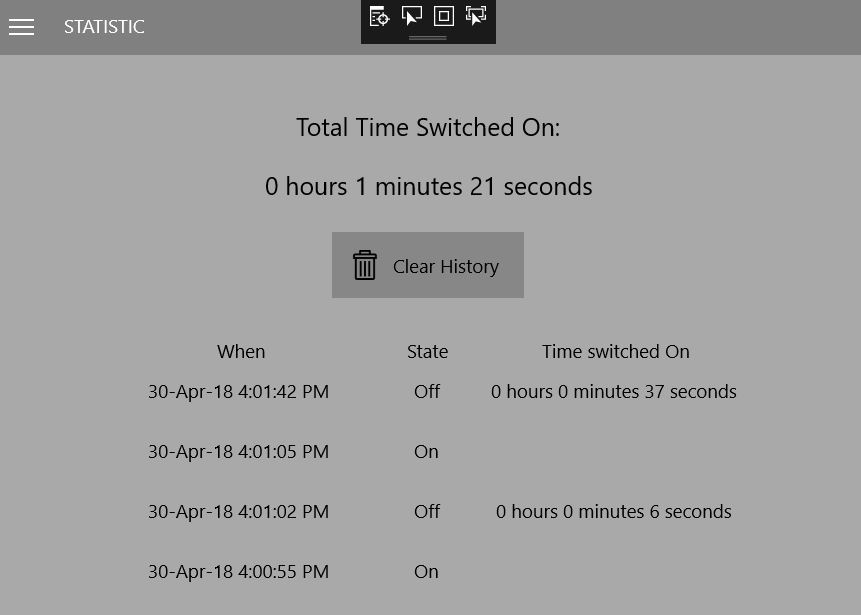
\includegraphics[width=\linewidth]{images/statisticview.jpg}
        \caption{Statisztika nézet}
    \end{subfigure}
    \begin{subfigure}[b]{0.4\linewidth}
        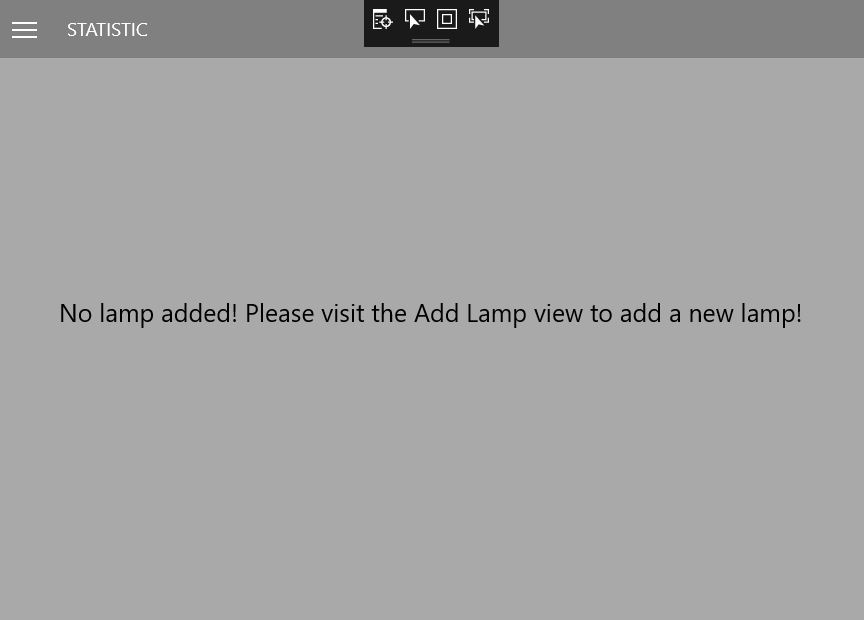
\includegraphics[width=\linewidth]{images/statisticnolamp.jpg}
        \caption{Statisztika nézet, ha nincs lámpa}
    \end{subfigure}
    \caption{Statisztika oldal}
    \label{fig:Statistic}
\end{figure}

    Lehetőség nyílik a teljes előzményt törölni, ez akkor lehet hasznos, ha például új villanykörtét szerelünk a lámpába,
    és szeretnénk ha tiszta lappal indulna a statisztika. Ehhez a ``Clear History'' feliratú gombra kell kattintatunk, ezután
    a korábbi esetekhez hasonlóan egy felugró ablak kéri a törlés megerősítését, a ``Yes'' opciót választva a sikeres törlés
    esetén visszaigazolást kapunk a művelet zökkenőmentes befejezéséről.

\begin{figure}[H]
    \centering
    \begin{subfigure}[b]{0.4\linewidth}
        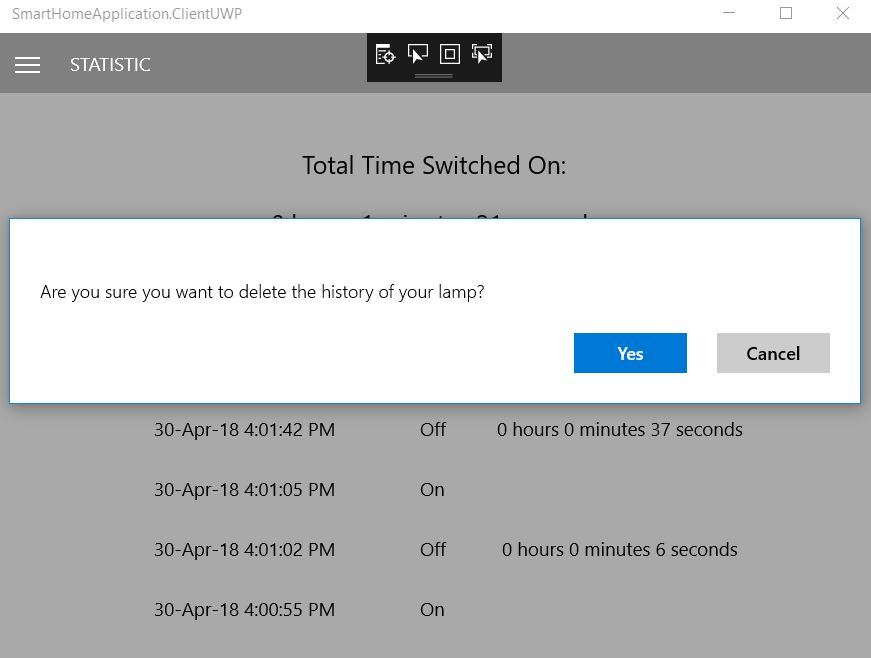
\includegraphics[width=\linewidth]{images/statistichistoriydeletesure.jpg}
        \caption{Előzmények törlésének megerősítése}
    \end{subfigure}
    \begin{subfigure}[b]{0.4\linewidth}
        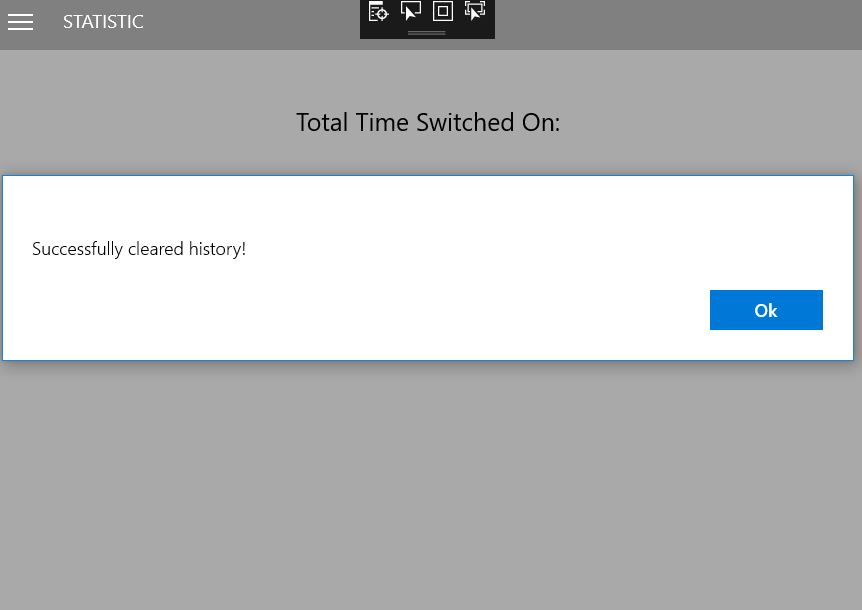
\includegraphics[width=\linewidth]{images/statisticdeletesucces.jpg}
        \caption{Előzmények törlése sikeresen lezajlott}
    \end{subfigure}
    \caption{Statisztika előzmények törlése}
    \label{fig:StatisticDelete}
\end{figure}

    \textbf{Fontos!} A törlés végleges, az előzményeket \textbf{nem} lehet visszanyerni, valamint ezen lámpa összes felhasználója
    számára törli az adatokat.

\subsubsection{Kijelentkezés}
    A felhasználó ki tud jelentkezni az alkalmazásból, a program a nevét és profilképét nem használja tovább. A menü alján
    található ``Log Out'' feliratú gomb egy kis ajtó ikonnal mellette. Erre kattintva a program egy szokásos felugró ablakkal
    győződik meg szándékunk komolyságáról. Megerősített kijelentkezés után a bejelentkező képernyőre navigál az alkalmazás.

\begin{figure}[H]
    \centering
    \begin{subfigure}[b]{0.4\linewidth}
        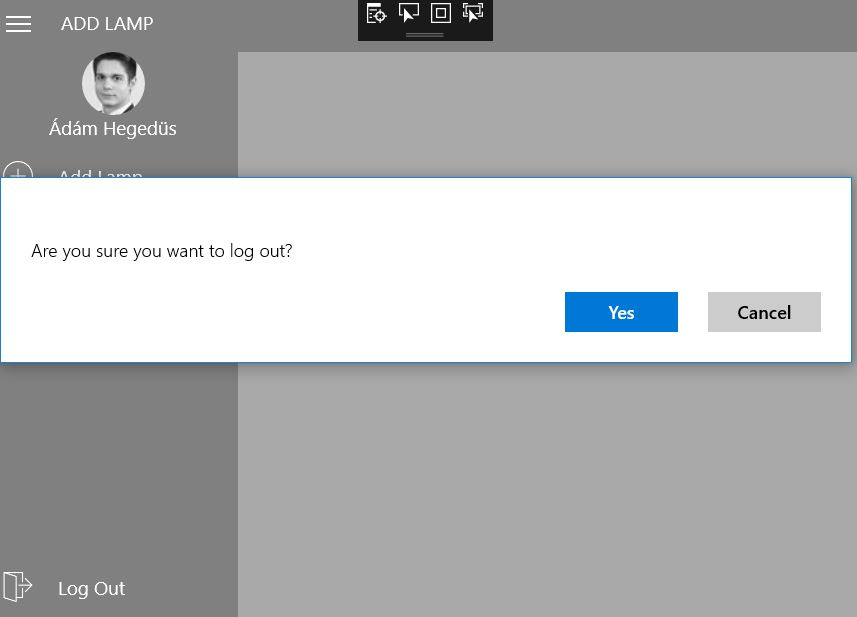
\includegraphics[width=\linewidth]{images/logoutsure.jpg}
        \caption{Kijelentkezés megerősítése}
    \end{subfigure}
    \begin{subfigure}[b]{0.4\linewidth}
        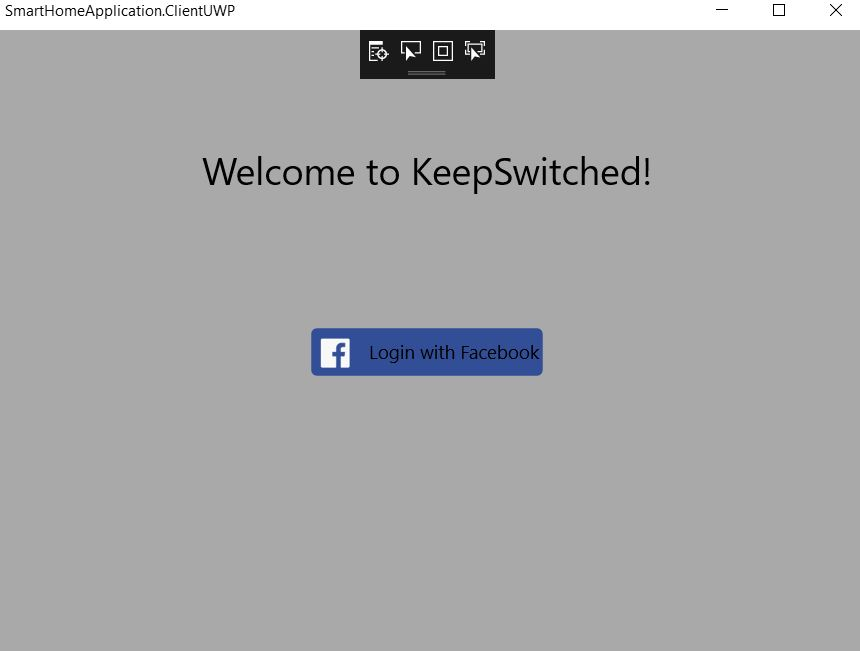
\includegraphics[width=\linewidth]{images/logoutbacktologin.jpg}
        \caption{Kijelentkezés után a bejelentkező oldal jelenik meg}
    \end{subfigure}
    \caption{Kijelentkezés menete}
    \label{fig:Logout}
\end{figure}

\chapter{Fejlesztői dokumentáció}

\section{Általános áttekintés}
    A program három fő részből áll, és mindegyik rész Microsoft technológiák felhasználásával készült. Kliens oldalon két
    Universal Windows Platform alkalmazás található. Az egyik, IoT kliensalkalmazás, mely egy Windows 10 IoT Core operációs rendszerrel
    telepített Raspberry Pi 3 Model B-n fut, feladata a rácsatlakoztatott lámpa vezérlése. A másik, egy Windows 10 asztali és mobil
    alkalmazás, mely az ügyfelek számára nyújt kényelmes felületet a fényforrás irányításához. Az előbbi két alkalmazást egy .NET Web
    szerver köti össze, mely Microsoft Azure App Service szolgáltatásában fut. Az adatbázist egy Azure SQL szerver testesíti meg, és a webes
    applikáció kezeli.

\begin{figure}[H]
    \centering
    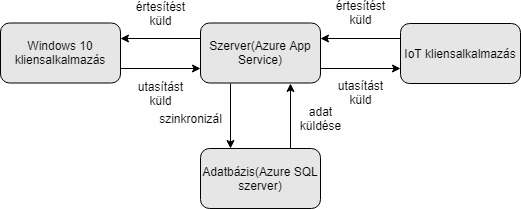
\includegraphics[width=\linewidth]{images/struktura.jpg}
    \caption{A program struktúrája}
    \label{fig: Struktura}
\end{figure}

\section{Követelmények}

\subsection{Hardver}
    A program elkészítéséhez az alábbi konfigurációt használtam:

\begin{itemize}
    \item Intel Core i7-7500U 2.70GHz
    \item 8 GB DDR4 RAM
    \item 256 GB SSD
    \item 2 db FullHD felbontású képernyő
\end{itemize}

    Ez az összetétel elegendőnek bizonyult, ennél gyengébb hardveren is elfuthat, azonban a fejlesztőkörnyezet erőforrásigénye
    miatt az alábbi \textbf{minimum} buildet javaslom:

\begin{itemize}
    \item Intel Core i5 processzor
    \item 256 GB SSD
    \item 16 GB RAM
\end{itemize}

\subsection{Szoftver}
    Az alábbi szoftverek szükségesek a program elkészítéséhez:

\begin{itemize}
    \item Windows 10 operációs rendszer
    \item Visual Studio 2017 Enterprise Edition
    \item Azure SDK
    \item LaTeX a dokumentáció elkészítéséhez
    \item Git a verziókezeléshez
\end{itemize}

\section{Forráskód letöltése}

\subsection{Verziókezelés}

\subsubsection{Git}
    A program verziókezeléséhez Git-et használtam, mely talán a legismertebb ilyen program a piacon. Lényege, hogy a forráskódot
    nem csak a számítógépünkön, hanem egy felhőben lévő tárhelyen, úgynevezett ``\textbf{repository}''-ban is tároljuk. Innen
    más is letöltheti, együtt lehet dolgozni a kódon, felügyelhetjük a másik fejlesztő munkáját, és a tárhelyen megtalálhatóak lesznek a
    biztonsági mentéseink is a szoftverről. Összehangolt fejlesztés elképzelhetetlen lenne ilyen verziókezelő programok nélkül.
    Tárhelyszolgálatásnak én \textbf{GitHub}-ot választottam, mely részben ingyenes, könnyen kezelhető, kényelmes felületet nyújt.

    A verziókezelő által nyújtott lehetőségek tárháza óriási, érdemes a hivatalos dokumentációt végigolvasni, hogy képet kapjunk arról,
    milyen parancsok léteznek, milyen kapcsolókat használhatunk hozzájuk. A dokumentáció a következő linken érhető el: \url{https://git-scm.com/docs}

\subsubsection{Git telepítése}
    A Git egyszerűen telepíthető verziókezelő program, mely hivatalos forrásból letölthető. Az \url{https://git-scm.com/download/win} oldalon
    letölhetjük a számunkra megfelelő Windows-os verziót. Kövessük a telepítő utasításait, a szoftver rövid időn belül feltelepül számítógépünkre.

\subsubsection{GitHub}
    Ahhoz, hogy le tudjuk tölteni a forráskódot a tárhelyről, szükséges regisztrálnunk az adott oldalra. Az \url{https://github.com/} oldalon
    a jobb felő sarokban található ``Sign Up'' feliratra kattintva hozhatunk létre új profilt. Ha rendelkezünk az egyetem által kibocsátott
    email címmel, akkor jogosultak vagyunk fizetős szolgáltatások ingyen elérésére, például privát tárhelyet hozhatunk létre.

\subsection{Tárhely klónozása}
    Git segítségével lehet ``klónozni'' a tárhelyet, vagyis a respository-ban lévő könyvtárat egy az egyben letölti az általunk kijelölt
    mappába. Miután sikeresen feltelepítettük a Git megfelelő verzióját, az alábbi lépéseket kell tennünk:

\begin{enumerate}
    \item Navigáljunk a könyvtárba, ahova szeretnénk a forráskódot letölteni
    \item Nyissunk meg egy parancssort
    \item Gépeljük be: git clone ``https://github.com/hegedusadam/SmartHomeApplication.git'', majd üssünk entert
    \item A program a GitHub felhasználónevünket és jelszavunkat fogja kérni
\end{enumerate}

\section{Microsoft Azure}
    Az Azure a Microsoft felhőalapű platformja, melyen infrastruktúra -és platformszolgáltatásokat vehetünk igénybe. Több mint
    hatszáz lehetőség közül választhatunk, számunkra azonban csak kettőre van szükség. Az \textbf{Azure App Service} és az
    \textbf{Azure SQL szerver} szolgáltatásokra. Ezek igénybevételéhez regisztrálnunk kell a \url{portal.azure.com} oldalon.
    Számos adatunk mellett bankkártya információkat is meg kell adnunk, azonban az App Service számunkra elegendő szolgáltatás
    ingyenes, az SQL szerver pedig minimális költséggel jár havonta, amennyiben egy gyengébb konfigurációt választunk.

\subsection{App Service létrehozása}
    Miután sikeresen regisztráltunk az oldalon, hozzuk létre a szerver futtatásához szükséges platformszolgáltatást. Kattintsunk
    a bal felső sarokban található ``\textbf{Create Resource}'' gombra, majd a megnyíló ablakban a ``\textbf{Web + Mobile}'' lehetőségre.
    A szakdolgozathoz ``\textbf{Mobile App}'' - ot használtam, de lényegi különbség nincs a ``Web App'' - hoz képest.
    Ezt követően töltsük ki a szükséges adatokat, majd a platform konfigurálja nekünk a szervert.

\begin{figure}[H]
    \centering
    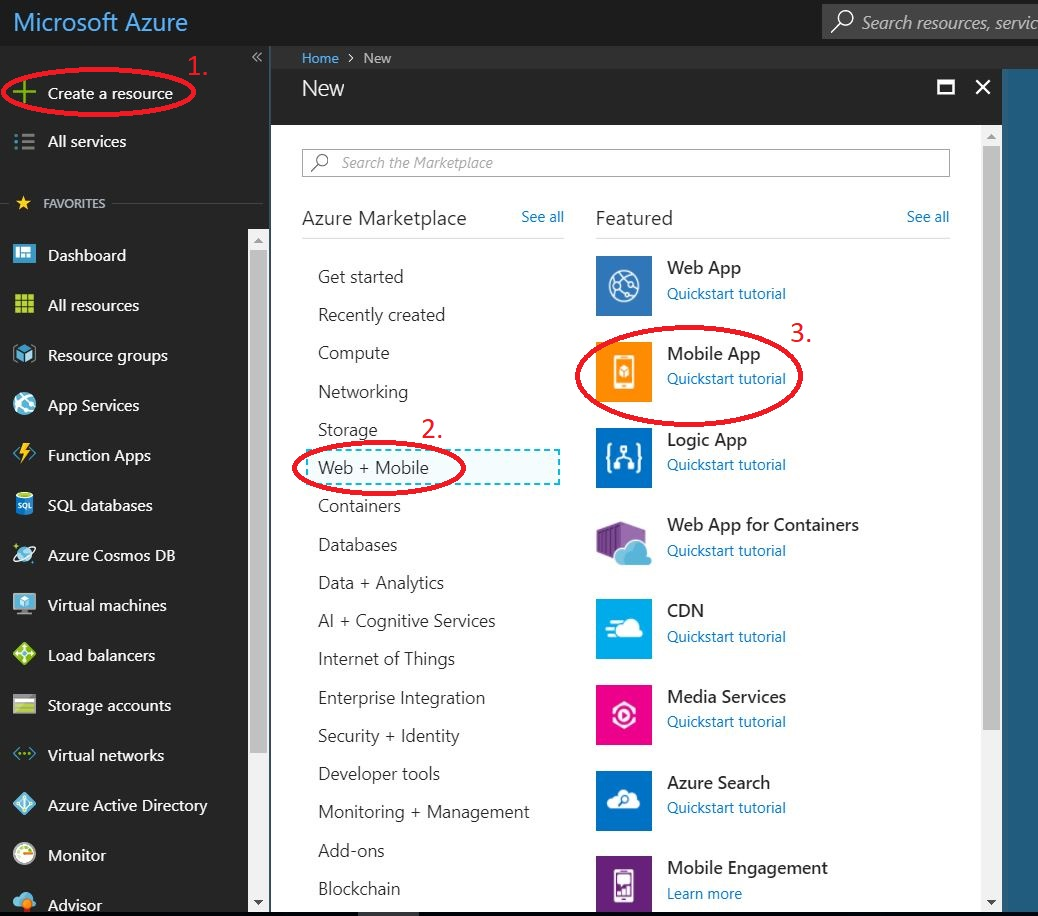
\includegraphics[width=10cm,keepaspectratio]{images/azurecreatemobilapp.jpg}
    \caption{Mobile App létrehozás lépései}
    \label{fig: MobileApp}
\end{figure}

\subsection{Azure SQL adatbázis létehozása}
    Az Azure adatbázis szolgáltatását fogjuk igénybe venni, mivel könnyen kezelhető, kényelmes felülete nyújt, és egyszerűen
    csatlakoztathatjuk a korábban létrehozott \textbf{Mobile App} szolgáltatásunkhoz.
    Adatbázis hozzáadásához ugyanúgy a bal felső sarokban a ``Create Resource'' lehetőségre kell kattintanunk, és a ``Popular''
    fül alatt talán már meg is találhatjuk a szükséges szolgáltatást, ha mégsincs ott, akkor a kereső kezdjük el gépelni az ``SQL``
    betűket, majd az eredmények között válasszuk az ``\textbf{SQL database}'' opciót.
    Jelen esetben is töltsük ki a megfelelő adatokat, szükséges paramétereket, figyeljünk az díjszabásra, nehogy egy túlzottan drága
    szolgáltatást rakjunk össze.

\begin{figure}[H]
    \centering
    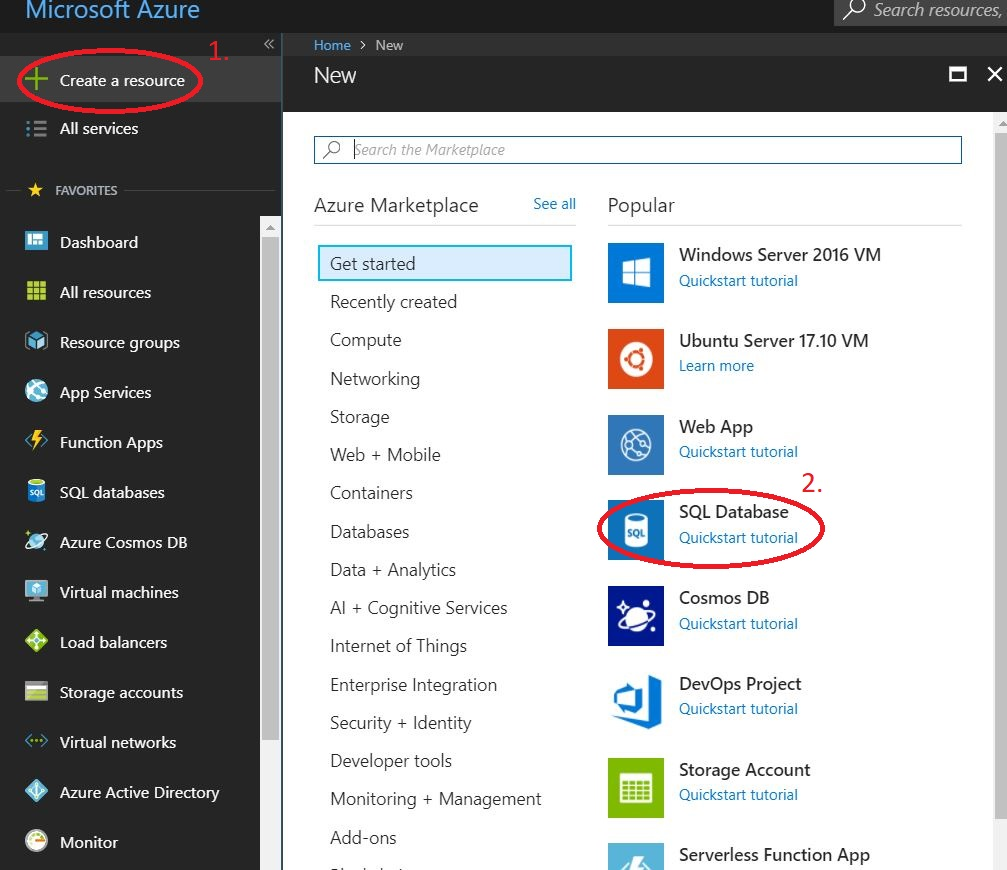
\includegraphics[width=10cm,keepaspectratio]{images/azuresqldatabase.jpg}
    \caption{SQL adatbázis létrehozás lépései}
    \label{fig: SQLDatabase}
\end{figure}

\subsection{Azure Active Directory}
    A Microsoft kész szolgáltatást nyújt Athentikációra is, lehetőségünk van valamelyik ismert közösségi oldal által nyújtott
    bejelentkezési felületet beleépíteni alkalmazásunkba. Ez azért előnyös, mert nem kell kritikus adat tárolásával foglalkoznom,
    elvégzi azt egy sokkal biztonságosabb szolgáltatás. A program elkészítéséhez Facebook authentikációt használtam, ezt be kell
    konfigurálni.
    Ehhez az alábbi lépések szükségesek:

\begin{enumerate}
    \item Lépjünk be a frissen létrehozott App Service vezérlőjébe. A lehetőségek között görgessünk le, amíg meg nem találjuk
    a kulcs ikonnal rendelkező \\ ``\textbf{Authentication/Authorization}'' menüpontot
    \item Állítsuk az ``\textbf{App Service Authentication}'' kapcsolót \textbf{On} - ra
    \item Az alatta lévő ``\textbf{Action to take when request is not authenticated}'' legördülő menüben válasszuk az
    ``\textbf{Allow Anonymous request}'' opciót. Azért engedélyezzük, mert az IoT kliensalkalmazásunk a GUID segítségével
    végzi az authentikációt, a kliensek által hívható függvényeknél használni fogjuk az Authenticate annotációt
    \item Jelen állás szerint a Facebook alatt a \textbf{Not Configured} feliratot kell látnunk. A közösségi oldal fejlesztőknek
    szóló oldalán kell további lépéseket tennünk, ehhez minden szükséges teendőt leír az alábbi hivatalos segítség:
    \url{https://docs.microsoft.com/en-us/azure/active-directory-b2c/active-directory-b2c-setup-fb-app}
    \item Az oldal legalján meg kell adnunk a \textbf{Redirect URL} - t, mely az előző pontban lévő konfigurációnál is kelleni fog.
    Példa url: \textbf{smarthomeapplicationservice://easyauth.callback}
\end{enumerate}

    Ha mindent jól csináltunk, akkor az Azure oldalán már nincs további teendőnk, még a szerver forráskódjában \textbf{szükséges}
    egy helyen változtatni, utána rendben fog működni az authentikáció. A Windows 10 kliensalkalmazás leírásában megtalálható a hátralévő változtatás.

\section{Az alkalmazás felépítése}
    Miután minden előzetes követelményt teljesítettünk, a szükséges szolgáltatásokat igénybe vettük, megfelelően konfiguráltuk,
    forráskódot letöltöttük, indítsuk el a \textbf{Visual Studio 2017} fejlesztőkörnyezetet, és nyissuk meg a \textbf{SmartHomeApplication}
    könyvtáron belül a \textbf{SmartHomeApplication.sln} fájlt, mely tartalmazza mindhárom rész forráskódját. Miután betöltött, a ``Solution Explorer'' - ben
    láthatjuk az egyes alkalmazásokat, azok felépítését, könyvtárait, osztályait. Ezen rész az előbb felsorolt dolgokat mutatja be
    részletesebben.

\begin{figure}[H]
    \centering
    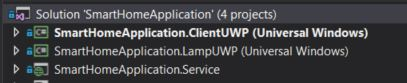
\includegraphics[width=8cm]{images/structure.jpg}
    \caption{Az alkalmazás alkotóelemei Solution Explorerben}
    \label{fig: SolutionExplorer}
\end{figure}

\subsection{Szerver}

\subsubsection{Áttekintés}
    A szerver egy ASP.Net webalkalmazás, mely C\# nyelven íródott, és végpontként szolgál. Ezen keresztül kommunikál a két kliensalkalmazás, és az adatbázissal
    is ő van kapcsolatban, szerepe kulcsfontosságú. A megvalósításhoz ASP.NET Web Api projekt sablont használtam, és \textbf{Model-View-Controller}
    (MVC) tervezési mintát. A Solution Explorerer - ben \textbf{SmartHomeApplication.Service} néven találhatjuk a projektet.

\subsubsection{Publish}
    Alkalmazásunkat még futtatnunk kell a már elkészített \textbf{Mobile App} - ban. Ezt könnyen megtehetjük Visual Studio - ban.
    Solution Explorer - ben kattintsunk jobb egérgombbal az alkalmazás nevére, majd a most megjelent lehetőségek közül válasszuk
    a ``\textbf{Publish}'' opciót. Ez egy másik oldalra fog navigálni, ahol ki kell töltenünk a szükséges adatokat, majd ha mindent
    megfelelően konfiguráltunk, akkor az alkalmazás hiba nélkül fog futni az App Service - ben.
    Mikor változtatunk a szerver forráskódján, akkor \textbf{kötelező} a Publish műveletet újra végrehajtani, azonban nincs szükség
    újra beállítani adatainkat.

    \textbf{Fontos!} A Publish beállításánál tudjuk pár lépésben hozzácsatolni a már korábban létrehozott SQL adatbázis szerverünket az alkalmazásunkhoz.

\begin{figure}[H]
    \centering
    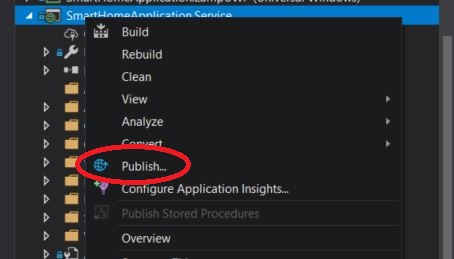
\includegraphics[width=8cm]{images/publishbutton.jpg}
    \caption{A Publish opciót válasszuk a lehetőségek közül}
    \label{fig: Publish}
\end{figure}

\subsubsection{Struktúra}
    Az alkalmazás számos generált könyvtár mellett az alábbi szükséges csomagokkal rendelkezik:

 \begin{itemize}
     \item \textbf{Models} - az adatbázis kapcsolatért és adatátvitelért felelős osztályok
     \item \textbf{Views} - megjelenítésért felelős osztályok
     \item \textbf{Controllers} - Az adatszolgáltatásért felelős végpontokat tartalmazó osztályok
     \item \textbf{Hubs} - A SignalR működéséhez szükséges \textbf{Hub} leszármazott osztályt tartalmazza
 \end{itemize}

\begin{figure}[H]
    \centering
    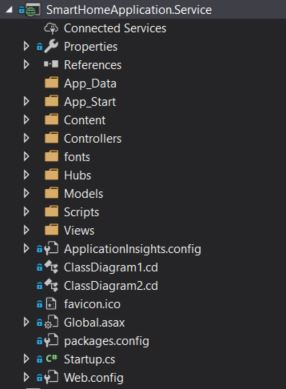
\includegraphics[width=6cm,keepaspectratio]{images/servicestructure.jpg}
    \caption{A szerver struktúrája}
    \label{fig: ServiceStructure}
\end{figure}

\subsubsection{Views}
    A megjelenítésért felelős osztályokat a \textbf{Views} package tartalmazza. Esetünkben a szervernek nincs szüksége
    felhasználói felületre, mivel végpontként funkciónál a kliensalkalmazások között, ezért a program \textbf{nem} tartalmaz
    ilyen osztályokat.

\subsubsection{Models}
    Az adatátvitelért és az adatbázis kapcsolatért felelős osztályok találhatóak meg ebben a csomagban, melyek az alábbiak:

\begin{itemize}
    \item \textbf{LampState.cs} - Ez egy \textbf{Data Transfer Object} (DTO) osztály, mely a változás hozzáadásához szükséges
    adatokat foglalja magába. Ezek a lámpa GUID-ja, a fel -vagy lekapcsolást jelentő logikai változó, illetve a DateTime típusú
    dátum
    \item \textbf{NewLamp.cs} - Szintén \textbf{DTO} osztály, mely egy lámpa felhasználóhoz csatlakoztatásához szükséges adatokat
    (UserId, GUID) foglalja magában
    \item \textbf{UserInfo.cs} - A harmadik \textbf{DTO} osztály, mely minden felhasználóval kapcsolatos adatot foglal össze, például
    UserId, az ügyfél lámpájának GUID-ja, neve, Facebook profilképének URI - ja.
    \item \textbf{SmartHomeApplicationDataBase.edmx} - A program Entity Framework - öt használ az adatbáziskezeléshez, ez a fájl
    tartalmazza a táblákat reprezentáló osztályokat, és azok grafikus megjelenítését.
\end{itemize}

\begin{figure}[H]
    \centering
    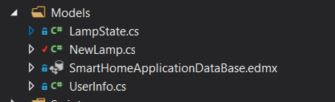
\includegraphics[width=6cm,keepaspectratio]{images/servicemodels.jpg}
    \caption{A Models csomag}
    \label{fig: ModelsPackage}
\end{figure}

\subsubsection{Controllers}
    A Controllers csomagban találhatóak azok az osztályok, melyek az adatok szolgáltatására hivatottak a két kliensalkalmazás irányába.
    Minden adatbázis táblához tartozik egy Controller osztály. Controller ősosztályból származtatottak, Get, Post, Delete, Put HTTP
    művelettekel rendelkeznek. Az alábbi Controller osztályok találhatóak meg a szerveralkalmazásban:\\

    \textbf{UserController} - A ``\textbf{Users}'' táblához tartozó Controller osztály, mely az ügyfelekkel kapcsolatos adatokat szolgáltatja
    elsősorban a Windows 10 kliensalkalmazás felé. Az alábbi végpontokkal rendelkezik:

\begin{figure}[H]
    \centering
    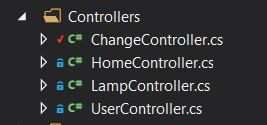
\includegraphics[width=6cm,keepaspectratio]{images/servicecontrollers.jpg}
    \caption{Controllers könyvtár. A HomeController egy használaton kívüli program által generált osztály}
    \label{fig: ControllersPackage}
\end{figure}

 \begin{itemize}
     \item \textbf{GetGuid} - \textbf{HttpPost} egy \textbf{UserInfo} objektumot kap paraméterül, feladata hogy visszaadja a paraméter
     objektum UserProfileId adattagjával megegyező \textbf{User} entitás lámpájának GUID - ját. Ha nincs csatlakoztatva eszköz,
     akkor egy konstans ``NOGUID'' karakterláncot ad vissza.
     \item \textbf{Register} - \textbf{HttpPost} egy \textbf{UserInfo} objektumot kap paraméterül, benne a felhasználó nevével és UserProfileId - vel
     , ezen adatokkal regisztrálja az új ügyfelet az adatbázisba ha még nem szerepel benne
     \item \textbf{GetUserInfo} - \textbf{HttpGet} feladata a Facebook megfelelő oldaláról lekérni a felhasználó nevét, és avatar URI - ját.
     Visszatérési értéke egy szerializált UserInfo objektum. Segédfüggvénye a \textbf{GetAccesToken}, mely
 \end{itemize}

    \textbf{ChangeController} - A ``\textbf{Changes}'' adatbázis táblához tartozó Controller osztály, mely a lámpák változásait kezeli az adatbázisban.
    Az alábbi két végponttal rendelkezik:

 \begin{itemize}
     \item \textbf{AddChange} - \textbf{HttpPost} egy \textbf{LampState} objektumot kap paraméterül, feladata hogy rögzítsen egy új állapotváltozást
     az adatbázisban a paraméter objektumban GUID adattagjához tartozó lámpához. A sikeres hozzáadás után az \textbf{IHubContext} adattag értesítést
     küld a klienseknek a változásról.
     \item \textbf{DeleteChanges} - \textbf{HttpPost} egy \textbf{string} paramétert kap, mely egy létező lámpa GUID - ját reprezentálja. A metódus
     törli a fényforásshoz tartozó összes változást, majd erről \textbf{IHubContext} segítségével értesítést küld a klienseknek.
 \end{itemize}

    \textbf{LampController} - A ``\textbf{Lamps}'' táblához tartozó Controller osztály, mely a lámpák kezeléséért felelős. Az itt lévő metódusok
    rendelnek lámpát egy felhasználóhoz, változtatják meg a lámpa állapot az adatbázisban majd küldenek erről értesítést a klienseknek. Ezen végpontok:

\begin{itemize}
    \item \textbf{AddUserToLamp} - \textbf{HttpPost} egy \textbf{NewLamp} objektumot kap paraméterül, mely egy UserId - t és egy GUID - ot tartalmaz.
    A GUID alapján megkeresi a \textbf{Lamp} entitást, mely \textbf{Users} adattagjához hozzáadja a UserId által meghatározott \textbf{User} - t.
    Rendelkezik \textbf{Authorize} annotációval, tehát csak bejelentkezett kliens tudja meghívni ezt az endpointot.
    \item \textbf{DeleteUserFromLamp} - \textbf{HttpPost} egy \textbf{UserInfo} objektumot kap paraméterül, mely a felhasználó userId - ját és
    a hozzá tartozó lámpának a GUID - ját tartalmazza. Feladata hogy eltávolítsa a lámpa Users adattagjából az adott ügyfelet, ezzel leválasztva
    a fényforrást a felhasználóról. Szintén \textbf{Authorize} annotációval rendelkezik, így csak és kizárólag sikeres bejelentkezés után
    lehet meghívni ezt a végpontot.
    \item \textbf{RegisterDevice} - \textbf{HttpPost} egy \textbf{string} paramétert kap, mely az új eszköz GUID - ja. Ezt a végpontot
    az IoT kliensalkalmazás hívja meg, mikor egy olyan mikroproccesszor futtatja az alkalmazást, mely még nincs jelen az adatbázisban,
    és ezzel regisztrálja magát.
    \item \textbf{TurnLamp} - \textbf{HttpPost} egy \textbf{bool} és egy \textbf{string} paramétert kap, a logikai változó a lámpa fel -vagy lekapcsolására
    szolgál, a karakterlánc pedig a kapcsolásra váró lámpa GUID - ját tartalmazza. Feladata az IoT kliensalkalmazást futtató eszközöknek
    jelet küldeni SignalR segítségével, hogy a megfelelő azonosítóval rendelkező lámpa végrehajtsa a változtatást. \textbf{Authorize}
    annotációval felruházott, tehát csak bejelentkezett felhasználók tudják meghívni.
    \item \textbf{GetChanges} - \textbf{HttpPost} egy \textbf{string} paramétert kap, mely egy eszköz azonosítóját takarja. A végpont visszaadja
    a GUID által reprezentált lámpa változásainak listáját, ami egy \textbf{ICollection}. \textbf{Authorize} annotációval felszerelt, csak Facebook
    authentikáción sikeresen átesett felhasználók kliensalkalmazása hívhatja meg.
    \item \textbf{UpdateLamp} - \textbf{HttpPut} egy \textbf{LampState} objektumot kap paraméterül, melyben a lámpa GUID - ját fedő \textbf{string}
    illetve az állapot reprezentáló \textbf{bool} adattag található. A végpontot az IoT kliensalkalmazás hívja meg, feladata felülírni az adatbázisban
    az adott eszköz \textbf{IsOn} mezőjét.
\end{itemize}

\subsubsection{Hubs}
    A valósidejűség megvalósítása érdekében a szerver használja a \textbf{Microsoft.AspNet.\\SignalR} könyvtárat, mely segítségével
    tud jelzést küldeni az eseményekre feliratkozott klienseknek. Ehhez szükség van egy \textbf{IHubContext} adattagra a Controller
    osztályokban, ezek példányosításához, pedig egy \textbf{LampHub} osztályra, mely \textbf{Hub} leszármazott. A valósidejűségről
    a későbbiekben még bővebben szó esik.

\subsection{IoT kliensalkalmazás}
    Az IoT kliensalkalmazás egy \textbf{Universal Windows Platform} alkalmazás, melynek sajátossága, hogy minden Windows 10 rendszerrel
    ellátott eszközön fut, így a Windows 10 IoT Core operációs rendszerrel felszerelt Raspberri Pi 3 Model B - n is. A program \textbf{C\#} nyelven
    íródott, a felhasználói felület pedig \textbf{XAML} - ben. Az alkalmazás \textbf{Model - View - ViewModel} (MVVM) tervezési mintát
    valósít meg, ám lokális adatbázissal nem rendelkezik, a szerveren keresztül kommunikál a tárhellyel. A ``Solution Explorer'' - ben
    \textbf{SmartHomeApplication.LampUWP} néven találjuk az alkalmazást.

\subsubsection{Struktúra}
    Az alkalmazás az MVVM tervezési minta alapján az alábbi részekkel rendelkezik:

\begin{itemize}
    \item \textbf{Model} - lokális adatbázissal nem rendelkezik az alkalmazás, de DTO osztályokat tartalmaz
    \item \textbf{View} - A GUID felület megjelenítésére szolgáló osztály
    \item \textbf{ViewModel} - a szerverrel való kapcsolattartás, a View számára állítja elő a megjelenítendő adatot
\end{itemize}

\subsubsection{Model}
    Lokális adatbázis nem léte miatt, a Model csomagban csak két darab \textbf{DTO} osztály található, melyek az alábbiak:

\begin{itemize}
    \item \textbf{GuidDTO} - egy \textbf{string} adattagot tartalmaz, mely az eszköz GUID - ját tartalmazza, az osztályt
    a \textbf{RegisterDevice} használja
    \item \textbf{LampStateDTO} - egy \textbf{string}, \textbf{bool}, és egy \textbf{DateTime} adattagot tartalmazó DTO
    osztály. Feladata, hogy az alkalmazás a lámpa állapotában történő változást közölje a szerver felé
\end{itemize}

\subsubsection{View}
    Az alkalmazás egyetlen \textbf{XAML} kiterjesztésű fájlt tartalmaz, \textbf{MainPage.xaml} néven, egyszerű felületet
    ír le, csupán két darab \textbf{TextBlock} található rajta egy \textbf{StackPanel} - en belül. Szerepe mégis kulcsfontosságú,
    megjeleníti, a lámpa GUID - ját, melyet a felhasználó innen leolvas, és hozzá tudja adni a profiljához a Windows 10 kliensalkalmazásban.

\subsubsection{ViewModel}
    A MainPage.xaml - hez tartozó ViewModel osztályt a projektben \textbf{MainViewModel.cs} néven lehet megtalálni. Ez az osztály
    felelős a szerverrel való kommunikációért, a megjelenítendő adat előállítása a View számára. Az osztály \textbf{GalaSoft.MvvmLight.ViewModelBase}
    leszármazott, megvalósítja az \textbf{INotifyPropertyChanged} interfészt.\\

    \textbf{Property - k} - A MainViewModel.cs az alábbi adattagokkal rendelkezik:

\begin{itemize}
    \item \textbf{LampGuid} - \textbf{string property}, mely a lámpa GUID - ját tárolja, szolgáltatja a View - nek
    \item \textbf{GpioController} - \textbf{GpioController property}, mely arra szolgál, hogy megnyissogn egy \textbf{LedPin} - t, így
    lehessen azt vezérelni
    \item \textbf{LedPin} - \textbf{LedPin property} a GPIO pin, melyen keresztül áramot tudunk vezetni a lámpába
    \item \textbf{OpenedPin} - \textbf{readonly int} konstans, mely a megnyitandó GPIO pin számát tartalmazza
\end{itemize}

    \textbf{Metódusok} - A MainViewModel osztály az alábbi metódusokkal rendelkezik:

 \begin{itemize}
     \item \textbf{Konstruktor} - az osztály tartalmaz egy paraméter nélküli konstruktort, melyben a \textbf{GpioController adattag} kap értéket,
     majd megnyitja az \textbf{OpenedPin} konstans adattag által megadott \textbf{LedPin} - t.
     \item \textbf{CreateOrReadGuid} - ez egy \textbf{public async Task} metódus, mely egy kulcs alapján ellenőrzi, hogy az adott eszköz
     rendelkezik-e már GUID - dal, vagy sem. Ha nem, akkor az \textbf{Application.Current.LocalSettings} segítségével a lokális könyvtárba
     a \textbf{Guid.NewGuid()} statikus metódussal generál egy új azonosítót a megadott kulccsal, így a legközelebbi indításkor már ezt az értéket
     fogja kiolvasni az alkalmazás a \textbf{LampGuid} property - be. A függvényt a \textbf{MainPage.xaml.cs} osztály konstruktorában hívódik meg.
     \item \textbf{RegisterDevice} - egy \textbf{private async Task} metódus, mely egy string paramétert kap, ami az eszköz GUID - ját tartalmazza.
     A függvény egy \textbf{HttpClient} segítségével meghívja a szerver \textbf{/Lamp/RegisterDevice} végpontját a kapott karakterlánccal, így
     a lámpa be lesz regisztrálva az adatbázisba. A függvényt a \textbf{CreateOrReplaceGuid} metódus hívja meg, miután új azonosítót generál.
     \item \textbf{SetupHub} - \textbf{public async Task} függvény, mely feliratkozik a szerver által fenntartott \textbf{Hub} - ra, azon belül
     az ``\textbf{OnSwitch}'' eseményre, mely a lámpa fel -és lekapcsolását kommunikálja a kliensek felé. A függvény függvény aszinkron módon hívódik
     meg a \textbf{MainPage.xaml.cs} osztály konstruktorában.
     \item \textbf{SwitchLamp} - \textbf{private async void} egy \textbf{string} és egy \textbf{bool} paraméterrel rendelkező függvény, mely az ``OnSwitch''
     esemény bekövetkezésekor lefut. Ellenőrzi, hogy a string paraméter által reprezentált GUID megegyezik-e a \textbf{LampGuid} property - vel. Ha nem,
     a metódus visszatér és semmi nem történik, ha igen akkor pedig a logikai változótól függően áramot vezet lámpába, vagy áramtalanítja azt.
     \item \textbf{SendLampState} - \textbf{private async Task} metódus, melyet a SwitchLamp függvény hív meg a sikeres állapotváltozás után.
     Feladata, hogy tájékoztassa a szervert az operáció végeztéről, így egy LampStateDTO objektumot készít a megfelelő adatokkal, majd azt szerializálja
     és egy \textbf{HttpClient} segítségével paraméterként elküldi a \textbf{/Lamp/UpdateLamp} és \textbf{/Change/AddChange} végpontokra.
 \end{itemize}

 \subsection{Windows 10 kliensalkalmazás}
    A Windows 10 kliensalkalmazás szintén egy \textbf{Universal Windows Platform} (UWP) alkalmazás, így a program bármely Windows 10
    operációs rendszerrel telepített eszközön fut, tehát mind asztali számítógépen, okostelefonon, vagy tableten. Az alkalmazás \textbf{C\#} nyelven
    íródott, a felhasználói felület elkészítéséhet pedig \textbf{XAML} - t használtam. Az IoT kliensalkalmazáshoz hasonlóan, a szakdolgozatom
    ezen része is \textbf{Model - View - ViewModel} (MVVM) tervezési mintát valósít meg, ám ennél az alkalmazásnál sem található lokális
    adatbázis, közvetlenül a szerveren keresztül szerzi az adatokat. Nyissuk meg a ``Solution Explorer'' - ben a \textbf{SmartHomeApplication.ClientUWP}
    projektet.

 \subsubsection{Struktúra}
    Az alkalmazás az alábbi szükséges könyvtárakkal rendelkezik, köztük a tervezési minta által meghatározottakkal:

\begin{itemize}
    \item \textbf{Assets} - az alkalmazás által használt képeket tartalmazza
    \item \textbf{Controls} - a felhasználó felület tervezésében használt \textbf{UserControl} - kat tárol
    \item \textbf{Converters} - a felhasználói felületen használt Converter osztályokat foglalja magában
    \item \textbf{Model} - a tervezési mintának megfelelő csomag, azonban lokális adatbázist nem tárol, kizárólag \textbf{DTO} osztályokat
    \item \textbf{Resources} - a felhasználói felület egységesítését elősgető \textbf{XAML} állományok, színeket, stílusokat tárolnak
    \item \textbf{View} - a felhasználói felület \textbf{XAML} állományait tartalmazza
    \item \textbf{ViewModel} - a tervzési mintának megfelelő csomag, a felhasználói felület számára adatot előállító és a szerverrel
    kommunikáló osztályokat tartalmazza
\end{itemize}

\subsubsection{Assets}
    Az alkalmazás számos képet használ, többek között a menüben, például hozzáadás, törlés ikon. Ezeket az Assets csomagban tárolja a program,
    azon belül három könyvtárra tagolva. A \textbf{SplitView} package - ban a menüben felhasznált képek találhatóak, a \textbf{Login} mappában
    a bejelentkezési felületen megtalálható Facebook logó van, a \textbf{Common} könyvtárban pedig az alkalmazás több részén előforduló ikonok,
    például a törlés gombok mellette található kuka ikon foglal helyet.

\subsubsection{Controls}
    Olyan elemeket tartalmazó \textbf{XAML} állományok, mely többször felhasználásra kerülnek, kiszervezésük külön fájlba egyszerűsíti a kódot
    és átláthatóbbá teszi azt. Két darab ilyen \textbf{UserControl} szerepel a csomagban, \textbf{SplitViewButtonContent.xaml} és
    \textbf{ViewButtonContent.xaml}.\\

    \textbf{SplitViewButtonContent} - A menü gombjait leíró állomány, mely egy \textbf{StackPanel} - en belül tárol egy \textbf{Image} - t,
    és egy \textbf{TextBlock} - ot. Például az ``Add Lamp'' menüpontnál látható egy bekarikázott plusz jel(Image), és maga az ``Add Lamp''
    szöveg, melyet a TextBlock tartalmaz.\\

    \textbf{ViewButtonContent} - Ugyanazon elemmekkel rendelkezik, mint a SplitViewButtonContent, azonban ennek az állománynak nincs
    ``\textbf{SelectedTextColor}`` illetve ``\textbf{SelectedImageSource}'' adattagja.

\subsubsection{Converters}
    A Converterek nagyon fontos szerepet játszanak a felhasználói felület működésében. Egy kapott paramétert alakítanak más típusú
    változóvá. Az alkalmazás négy darab konvertáló osztály tartalmaz, melyek megvalósítják az \textbf{IValueConverter} interfészt:\\

    \textbf{BooleanToOnOrOffStringConverter.cs} - egy \textbf{bool} értéket kap paraméterül, ez alapján ad vissza egy ``On'' vagy
    ``Off'' stringet. A \textbf{StatisticView} oldal használja, mikor a táblázatban meg kell jeleníteni, hogy egy adott változás
    alkalmazával a lámpát be (``On'')  -vagy lekapcsolták. (``Off'')\\

    \textbf{NoGuidToCollapsedVisibilityConverter.cs} - egy \textbf{string} paramétert kap, ebből kell előállítania \textbf{Visibility} értéket.
    Ezt a Convertert a lámpával kapcsolatos oldalak használják, és a \textbf{LampGuid} alapján rejtik el vagy jelenítik meg
    a vizuális elemeket. Ha nincs lámpa csatolva a felhasználóhoz, akkor elrejti, ha van, akkor megjeleníti, például a kapcsolót.\\

    \textbf{NoGuidToVisibleVisibilityConverter.cs} - az előző Converter inverze. Szintén \textbf{string} paraméterből állít elő
    \textbf{Visibility} - t, hasonlóan a \textbf{LampGuid} adattag alapján, azonban ez az osztály akkor jeleníti meg az elemet,
    ha nincs lámpa csatolva a felhasználóhoz, tehát a LampGuid ``NOGUID'' értékkel rendelkezik. Ezt a konvertálót használják azok az
    elemek, melyek tájékoztatnak a hozzáadott eszköz hiányáról, például a \textbf{LampSwitchView} állományban.\\

    \textbf{TimeSpanToStringConverter.cs} - szintén a \textbf{StatisticView} használja a táblázaton belül, feladata hogy egy \textbf{TimeSpan}
    objektumból a felhasználó számára kényelmesen leolvasható információt alakítson. A TimeSpan méri két \textbf{DateTime} közt eltelt
    időt, ebből formáz órákra, percekre, másodpercekre lebontott eredményt.

\subsubsection{Resources}
    Az alkalmazásban számos ismétlődő elem van. Színek, stílusok, ikonok, ezen tulajdonságok állandó ismétlése bonyolultságot
    és hibalehetősőséget adna a kódnak. Ezért érdemes ezeket kigyűjteni külön fájlokban, nevet adni neki, majd ez alapján hivatkozni
    rájuk a megfelelő elemekben, így sokkal átláthatóbb és kezelhetőbb lesz a forráskód. Kettő fájl található a csomagban:\\

    \textbf{Colors.xaml} - Különböző színkódokat tárol, melyeket több helyen felhasznál az alkalmazás, például: \textbf{ViewColor}.\\

    \textbf{Styles.xaml} - Különböző stílus leírásokat tárol, melyeket a program számos helyen felhasznál. A leírások több sorosak,
    így végtelen átláthatatlan lenne a kód ha nem gyűjtenénk ki őket külön fájlba. Példa: \textbf{SplitViewButtonStyle}.

\subsubsection{Model}
    A tervezési minta része, mely lokális adatbázis \textbf{nem} tárol, ez az alkalmazás is közvetlenül a szervertől kéri le az
    adatokat. \textbf{Data Transfer Object} osztályokat tartalmaz, melyek a kommunikációt teszik lehetővé a szerveroldallal.

\begin{itemize}
    \item \textbf{Change.cs} - a lámpa egy változását reprezentálja, tartalmaz \textbf{DateTime}, \textbf{bool}, \textbf{TimeSpan} property - ket,
    melyek segítségével a \textbf{StatisticView} fel tudja tölteni a táblázatot az oldalon.
    \item \textbf{UserInfo.cs} - a felhasználó adatainak megfelelő property - kel rendelkezik, melyek a ``userId''-t, az ügyfél nevét
    a lámpájának GUID -  ját, valamint Facebook profilképének Uri - ját tárolják.
\end{itemize}

\subsubsection{View}
    Ebben a csomagban találhatóak a megjelenítésért felelős \textbf{XAML} fájlok. Összesen öt darab állomány szerepel az alkalmazásban,
    ezek az alábbiek:

    \textbf{LoginView.xaml} - A felhasználó ezt az oldal látja először, ezen keresztül tud bejelentkezni az alkalmazásba. Egy \textbf{TextBlock} - ot
    tartalmaz, mely az üdvözlő szöveget tartalmazza, és egy \textbf{StackPanel} - t, melyen belül a bejelentkező gomb foglal helyet, mely egy további
    StackPanel - t tárol, amin belül az ikont megjelenítő \textbf{Image} és a gomb feliratát kiírató TextBlock található.  A gomb \textbf{Command}
    attribútumához hozzá van kötve a \textbf{LoginViewModel} LoginCommand property - je.

\begin{figure}[H]
    \centering
    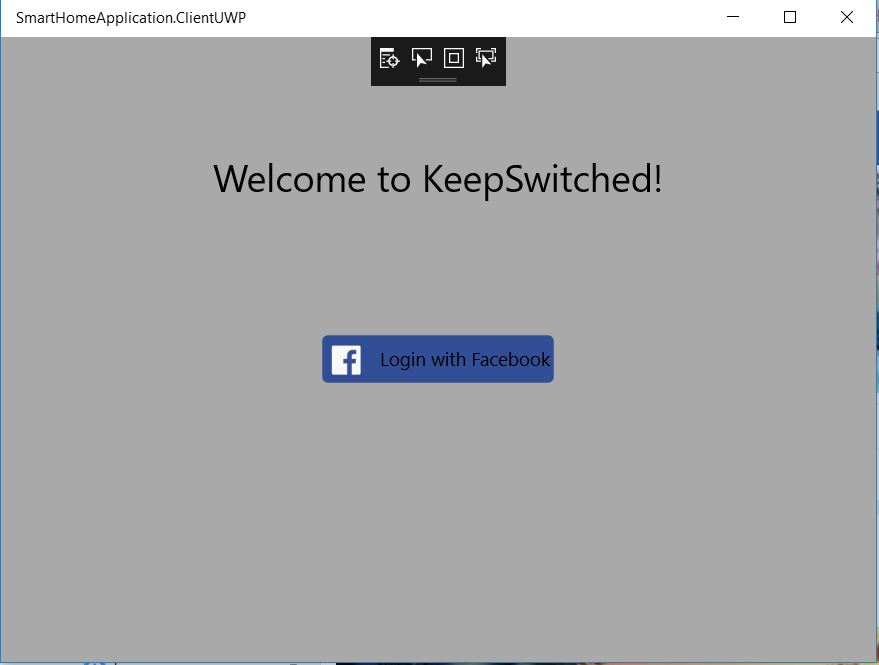
\includegraphics[width=6cm,keepaspectratio]{images/loginview.jpg}
    \caption{LoginView}
    \label{fig: LoginView}
\end{figure}

    \textbf{AddLampView.xaml} - Az az oldal mely a lámpa hozzáadására alkalmas felülete valósítja meg. Egy középre igazított \textbf{StackPanel} - t
    tartalmaz, melyben két darab \textbf{TextBlock}, egy \textbf{TextBox} - ot, valamint egy Button - t tartalmaz, amin belül egy \textbf{control:ViewButtonContent}
    található. Az egyik TextBlock \textbf{NoGuidToCollapsedVisibility} converterrel rendelkezik, tehát akkor jelenik meg, ha már hozzáadtunk lámpát,
    és erről tájékoztatja a felhasználót. A többi komponens mind \textbf{NoGuidToVisibleVisibilityConverter} - rel van felvértezve, és akkor
    jelennek meg mikor éppen nincs csatlakoztatott eszközünk. A TextBox - ba írhatjuk a GUID - ot, a gombbal pedig végrehajtani az \textbf{AddLampViewModel}
    ``AddLampCommand'' property - jét, mely a gombhoz van

\begin{figure}[H]
    \centering
    \begin{subfigure}[b]{0.4\linewidth}
        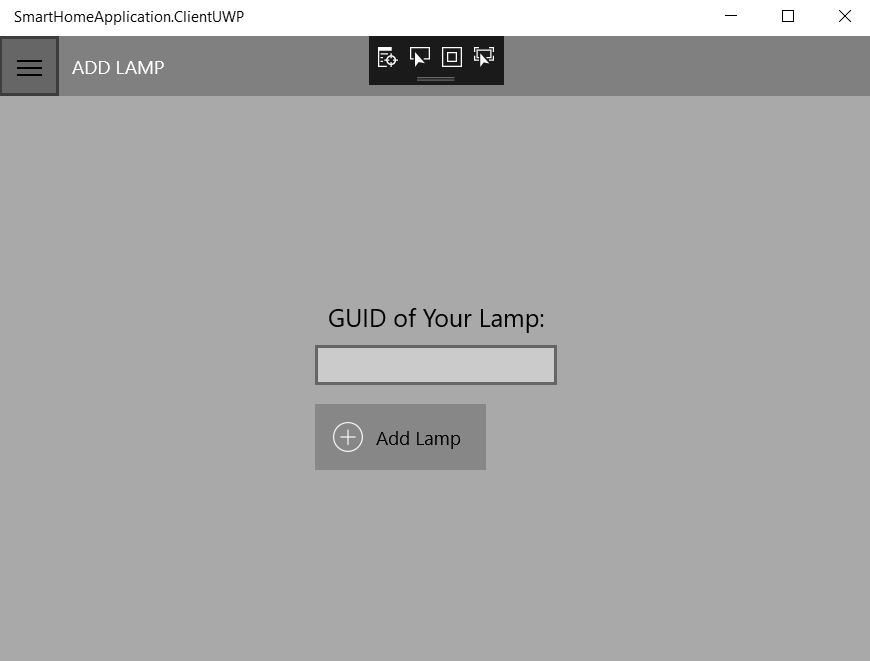
\includegraphics[width=\linewidth]{images/addlampview.jpg}
        \caption{AddLampView - nincs lámpa}
    \end{subfigure}
    \begin{subfigure}[b]{0.4\linewidth}
        \includegraphics[width=\linewidth]{images/alreadyhaslamp.jpg}
        \caption{AddLampView - van lámpa}
    \end{subfigure}
    \caption{AddLampView}
    \label{fig:AddLamp}
\end{figure}

    \textbf{LampSwitchView.xaml} - A lámpa vezérlésére alkalmas oldal. Három elemet tartalmaz, egy \textbf{ToggleSwitch} - et, mely
    egy szabályos kapcsoló, és ezzel lehet fel -vagy lekapcsolni a fényforrást, egy \textbf{controls:ViewButtonContent} - et, ami egy
    Button elemen belül található és az eszköz törlését lehet elindítani a hozzákötött \textbf{DeleteLampCommand} segítségével. Ezek
    \textbf{NoGuidToCollapsedVisibilityConverter} - rel rendelkeznek, míg a TextBlock az ellenkezőjével, az hívja fel a figyelmünk
    a lámpa hiányára.

\begin{figure}[H]
    \centering
    \begin{subfigure}[b]{0.4\linewidth}
        \includegraphics[width=\linewidth]{images/switchview.jpg}
        \caption{SwitchLampView - van lámpa}
    \end{subfigure}
    \begin{subfigure}[b]{0.4\linewidth}
        \includegraphics[width=\linewidth]{images/switchdonthavelamp.jpg}
        \caption{SwitchLampView - nincs lámpa}
    \end{subfigure}
    \caption{SwitchLampView}
    \label{fig:SwitchLamp}
\end{figure}

    \textbf{StatisticView.xaml} - A lámpa statisztikáit tekinthetjük meg ezen az oldalon. Egy \textbf{StackPanel} fogja közre a fő
    elemeket, melyek egy az összes bekapcsolt időt kiírató TextBlock, az előzményeket kitörlő \textbf{controls:ViewButtonContent} - et tartalmazó
    Button, melyhez a \textbf{StatisticViewModel} DeleteChangesCommand property - je van hozzákötve. Továbbá az oldal fő összetevője egy \textbf{ScrollViewer},
    amely az előzmények táblázatát testesíti meg. A most felsorolt elemek mind \textbf{NoGuidToCollapsedVisibilityConverter} - rel vannak ellátva,
    mivel csak akkor lehet statisztikát megtekinteni, ha van is eszköz aminek le lehet kérni az előzményét. Egy TextBlock jelenik meg a képernyőn a megfelelő
    szöveggel ha nem rendelkezünk eszközzel.

\begin{figure}[H]
    \centering
    \begin{subfigure}[b]{0.4\linewidth}
        \includegraphics[width=\linewidth]{images/statisticview.jpg}
        \caption{StatisticView - van lámpa}
    \end{subfigure}
    \begin{subfigure}[b]{0.4\linewidth}
        \includegraphics[width=\linewidth]{images/statisticnolamp.jpg}
        \caption{StatisticView - nincs lámpa}
    \end{subfigure}
    \caption{StatisticView}
    \label{fig:StatisticView}
\end{figure}

    \textbf{SplitViewShell.xaml} - Az alkalmazás kulcsfontosságú része. Erre navigál a program a sikeres bejelentkezés után, ez a nézet
    felelős a menü és a többi oldal megjelenítéséért. Egy \textbf{SplitView} - t tartalmaz, melynek két része van. Az egyik, melyben a hamburger
    menü van, nyitható, összecsukható, a másik az az oldal amit a menüpontok közül kiválaszt a felhasználó, vagy kezdetben az ``AddLampView''.
    A menüpontok \textbf{control:SplitViewButtonContent} -ket tartalmazó Button elemek, a kiválasztott gomb képe és szövegének háttere kék lesz.

\begin{figure}[H]
    \centering
    \includegraphics[width=6cm,height=7cm,keepaspectratio]{images/hamburgermenu.jpg}
    \caption{SplitViewShell}
    \label{fig: SplitViewShell}
\end{figure}

\subsubsection{ViewModel}
    A ViewModel osztályok kulcsfontosságúak a program működésében. Ők állítják elő a nézetek számára a szükséges adatokat, melyeket \textbf{DataBindig} - gal
    küldenek át a XAML fájloknak, valamint a szerverrel val kommunikációt is ők végzik. Az összes osztály \textbf{Galasoft.MvvmLight.ViewModelBase} leszármazott, így
    megvalósítják az \textbf{INotifyPropertyChanged} interfészt. Az alkalmazás az alábbi négy ViewModel osztállyal rendelkezik:\\

    \textbf{LoginViewModel.cs} - ez a LoginView - hoz tartozó ViewModel, tartalmazza az authentikáció szükséges eljárásokat. \\

    Két darab \textbf{property} - vel rendelkezik:

\begin{itemize}
    \item \textbf{LoginCommand} - \textbf{ICommand}, a LoginView bejelentkező gombjához van kötve, mikor a gombra kattint a felhasználó
    ez a parancs fut le, ami meghívja az \textbf{AuthenticateAsync} metódust.
    \item \textbf{IsLoggedIn} - \textbf{bool}, igaz, ha a felhasználó sikeresen bejelentkezett, különben hamis. Az \textbf{App.xaml.cs}
    állományban van szükség rá, a program nem fut tovább sikertelen authentikáció esetén.
\end{itemize}

    Az alábbi metódusok találhatóak meg benne:

\begin{itemize}
    \item \textbf{AuthenticateAsync} - \textbf{private async Task<bool>}, ez a metódus végzi az authentikációt. Az \textbf{App.xaml.cs} - ben
    található \textbf{MobileService} adattag \textbf{LoginAsync} függvényét hívja meg Facebook authentikációra. \\
    \\\textbf{Fontos!} - Az \textbf{Azure Active Directory} - val kapcsolatban volt még egy dolog amit szükséges változtatni a programon ha saját
    szerveren szeretnénk futtatni. A LoginAsync eljárás második paramétere egy string \textbf{UriScheme}, melynek meg kell egyeznie
    a \textbf{redirect url} első felével. Tehát a példánkban \textbf{smarthomeapplicationservice://easyauth.callback} volt az url,
    ezért az UriScheme \textbf{smarthomeapplicationservice} lesz, ahogy a kódban is látszik.\\
    \\Sikeres bejelentkezés után az IsLoggedIn property - t ``true'' értékre állítja, valamint meghívja a \textbf{GetUserInfo} metódust.
    \item \textbf{GetUserInfo} - \textbf{private async Task}, sikeres bejelentkezés után a metódus meghívja a \textbf{/User/GetUserInfo} végpontot,
    ezzel lekérve a felhasználó nevét, profilképét. Az eljárás két további fontos függvényt hív meg, \textbf{RegisterToDatabase} - t, és \textbf{GetLampGuid} - ot.
    \item \textbf{RegisterToDataBase} - \textbf{private async Task}, a felhasználót regisztrálja be az adatbázisba a neve és a \textbf{UserProfileId} - ja alapján.
    \item \textbf{GetLampGuid} - \textbf{private async Task}, lekéri a felhasználó lámpájának GUID - ját az adatbázisból, és elmenti
    az App.UserInformation adattagba, ahonnan később minden további ViewModel eléri.
\end{itemize}

    \textbf{AddLampViewModel.cs} - Az \textbf{AddLampView} - hez tartozó ViewModel osztály, feladata az új eszköz hozzáadásának
    folyamatát lefolytatni a szerverrel.\\
    Három \textbf{property} - vel rendelkezik:

\begin{itemize}
    \item \textbf{NewLampGuid} - \textbf{string} - a felhasználó által begépelt karaktersorozat, a hozzáadni kívánt eszköz azonosítója,
    melynek még át kell esnie ellenőrzéseken. (Megfelelő hossz, létező azonosító)
    \item \textbf{LampGuid} - \textbf{string} - a jelenlegi eszköz azonoítója
    \item \textbf{AddLampCommand} - \textbf{ICommand} - a parancs, mely az \textbf{AddLampView} lámpa hozzáadás gombjához van hozzárendelve,
    aktiváláskor meghívja az \textbf{AddNewLamp} függvényt
\end{itemize}

    \textbf{Metódusok} - az osztály egyetlen metódussal rendelkezik, az \textbf{AddNewLamp} eljárással, mely egy új eszköz hozzáadásását
    biztosítja. Előzetesen ellenőrzi hogy az ügyfél által begépelt \textbf{NewLampGuid} öt karakter hosszúságú-e. Ha nem, akkor egy
    \textbf{MessageDialog} ablak közli, hogy érvénytelen GUID - dal próbálkoztunk, majd a függvény visszatér. Az azonosító létezését
    a szerver ellenőrzi, nem a kliens feladata. Ha megfelelő hosszúságú a GUID, akkor az eljárás meghívja a \textbf{/Lamp/AddUserToLamp}
    végpontot. Az visszaad egy \textbf{HttpResponseMessage} - t, mely alapján eldönthető hogy a hozzáadás sikeresen zajlott - e le, és erről
    MessageDialog - ban tájékoztatja a felhasználót.\\

    \textbf{LampSwitchViewModel.cs} - A \textbf{LampSwitchView} - hoz tartozó ViewModel, feladata a lámpa állapotával kapcsolatos
    kommunikációt folytatni a szerverrel.\\

    Az alábbi \textbf{property} - kel rendelkezik:

\begin{itemize}
    \item \textbf{LampGuid} - \textbf{string}, a többi ViewModel - hez hasonlóan, ez az osztály is tárolja a lámpa GUID - ját, és törlés
    esetén meg is változtatja az \textbf{App} osztályban található property - t.
    \item \textbf{DeleteLampCommand} - \textbf{ICommand}, a törlés gombhoz kötött parancs, aktiváláskor meghívja a \textbf{DeleteLamp} metódust
    \item \textbf{IsOn} - \textbf{bool}, a \textbf{ToggleSwitch} - hez hozzákötött logikai változó, a kapcsoló állapota ettő a változótól függ
\end{itemize}

    \textbf{Metódusok:}

\begin{itemize}
    \item \textbf{Konstruktor} - az osztály konstruktora beállítja a LampGuid property - t, illetve egy külön szálon meghívja az \textbf{Initialize} eljárást.
    \item \textbf{Initialize} - \textbf{private async Task}, az osztály létrejöttekor lekéri a szervertől a lámpa állapotát, hogy a kapcsoló
    azonnal megfelelően működjön
    \item \textbf{SetupHub} - \textbf{public async Task}, ez a függvény felelős a \textbf{Hub} ``SwitchClient'' eseményére való feliratkozásért
    , így a kliens értesül a lámpa állapotában végbement változásokról
    \item \textbf{SwitchUponChange} - \textbf{private async void}, külső változtatás esetén ez a metódus fut le, mely ellenőrzi, hogy a lámpa
    azonosítója megegyezik-e a felhasználóéval, és ha igen, akkor állítja az \textbf{IsOn} property - t.
    \item \textbf{SwitchLamp} - \textbf{private async Task}, a felhasználó által végzett változtatást közli a szerver felé, meghívja a
    \textbf{/Lamp/TurnLamp} végpontot.
    \item \textbf{DeleteLamp} - \textbf{private async Task}, a lámpa eltávolítását végző metódus.  Egy \textbf{MessageDialog} - ban megerősítést
    kér az ügyféltől, majd meghívja a \textbf{/Lamp/DeleteUserFromLamp} végpontot, a sikeres törlés után tájékoztatja a felhasználót, majd
    eltávolítja a GUID - ot.
\end{itemize}

    \textbf{StatisticViewModel.cs} - A \textbf{StatisticView} - hez kapcsolódó ViewModel osztály, feladata a szervertől lekérni a lámpához
    tartozó változásokat, új változás esetén pedig frissíteni a felhasználói felületet.\\

    \textbf{Property - k:}

\begin{itemize}
    \item \textbf{DeleteChangesCommand} - \textbf{ICommand}, az előzményeket törléséért felelős gombhoz kötött parancs, mely meghívja a
    \textbf{DeleteChanges} metódust
    \item \textbf{LampGuid} - \textbf{string}, a felhasználóhoz tartozó lámpa azonoítója
    \item \textbf{TotalTimeOn} - \textbf{TimeSpan}, a teljes időmennyiséget tartalmazza, mialatt a lámpa be volt kapcsolba
    \item \textbf{ChangesCollection} - \textbf{ObservableCollection<Change>}, a változásokat tároló Collection, ezen adatok
    alapján készül a táblázat a felhasználói felületen.
\end{itemize}

    \textbf{Metódusok:}

\begin{itemize}
    \item \textbf{Konstruktor} - beállítja a LampGuid property - t, majd egy külön szálon meghívja az \textbf{Initialize} függvényt
    \item \textbf{Initialize} - \textbf{private async Task}, az osztály példányosításakor fut le, ha nincs GUID - ja a felasználónak akkor
    visszatér az eljárás, különben meghívja a \textbf{GetData} függvényt
    \item \textbf{SetupHub} - \textbf{public async Task}, feliratkozik a \textbf{Hub} ``ChangeAdded'' és ``ChangesDeleted'' eseményeire,
    melyekhez hozzáköti a \textbf{RefreshChanges} függvényt.
    \item \textbf{RefreshChanges} - \textbf{private async void}, a megfelelő esemény bekövetkezte után fut le ez a függvény, feladata
    újra lekérni az adatok a \textbf{GetData} eljárással.
    \item \textbf{GetData} - \textbf{private async Task}, meghívja a \textbf{GetChanges} függvényt, mely egy Change - ket tartalmazó
    \textbf{ICollection} - t ad vissza. Továbbá végrehajta a \textbf{GetMinutesOn} és \textbf{GetTotalTimeOn} eljárásokat a kapott eredményre.
    \item \textbf{GetChanges} - \textbf{private async Task<ICollection<Change>>}, ez a metódus kéri le a szervertől a lámpához tartozó változásokat a
    \textbf{/Lamp/GetChanges} végpont segítségével.
    \item \textbf{GetMinutesOn} - \textbf{private void}, végigiterál a Change - ket tartalmazó ObservableCollection - on, és minden eleménél
    kiszámolja, hogy mennyi idő telt el az őt megelőző elem \textbf{DateTime} adattagja által meghatározott dátum óta
    \item \textbf{GetTotalTimeOn} - \textbf{private TimeSpan}, végigiterál az ObservableCollection - on, és a Change - k \textbf{timeOn} adattagjait
    összegzi
    \item \textbf{DeleteChanges} - \textbf{private async Task}, törli a lámpa előzményeit a \textbf{/Change/DeleteChanges} végpont segítségével
    miután megerősítést kérta felhasználótól \textbf{MessageDialog} formában
\end{itemize}

\subsubsection{App.xaml.cs}
    Fontos kiemelni ezt az osztályt, mivel kulcsfontosságú szerepet játszik a program életében. Ez az alkalmazás belépési pontja,
    a keret méretét a konstruktor állítja be. A globális, ViewModellek által használt adattagok itt találhatóak, a felhasználó adatait
    tároló \textbf{UserInfo}, valamint az authentikációt, és a szerverrel való kommunikációt végző \textbf{MobileServicClient} is.
    Az alkalmazás indításakor a program ellenőrzi az internetkapcsolatot, az ehhez szükséges függvény itt található \textbf{hasInternetCollection}
    néven.

\section{Adatbázis bemutatása}
    Az adatbázis külön, összesen három táblában tárolja az adatokat, melyek az alábbiak:

\begin{figure}[H]
    \centering
    \includegraphics[width=\linewidth]{images/database.jpg}
    \caption{Az adatbázis felépítése}
    \label{fig: Database}
\end{figure}

\subsection{User}
    Ez a tábla felelős a felhasználók adatainak tárolásáért. A \textbf{Lamp} táblával \textbf{sok - egy} kapcsolatban áll. Az alábbi
    oszlopokkal rendelkezik:

\begin{itemize}
    \item \textbf{Id} - a tábla elsődleges kulcsa
    \item \textbf{FirstName} - a felhasználó keresztneve
    \item \textbf{LastName} - a felhasználó vezetékneve
    \item \textbf{UserProfileId} - felhasználó Facebook azonosítója
    \item \textbf{lampid} - idegen kulcs a \textbf{Lamp} táblához
\end{itemize}

\subsection{Change}
    Ez a tábla tárolja a lámpa változásait. \textbf{Sok - egy} kapcsolatban áll a \textbf{Lamp} táblával.

\begin{itemize}
    \item \textbf{Id} - a tábla elsődleges kulcsa
    \item \textbf{date} - a változás dátuma
    \item \textbf{state} - a változás állapota \textbf{False - kikapcsolva}, \textbf{True - bekapcsolba}
    \item \textbf{lampid} - idegen kulcs a \textbf{Lamp} táblához
\end{itemize}

\subsection{Lamp}
    Ez a tábla tárolja a lámpával kapcsolatos adatokat. A \textbf{User} és a \textbf{Change} táblával \textbf{egy - sok} kapcsolatban
    áll.

\begin{itemize}
    \item \textbf{Id} - a tábla elsődleges kulcsa
    \item \textbf{ison} - a lámpa aktuális állapota
    \item \textbf{lampguid} - az eszköz egyedi azonosítója
\end{itemize}

\section{Valósidejűség az alkalmazásban}
    Az alkalmazás fő tulajdonsága, hogy valós időben értesülünk az eseményekről. Mit is jelent ez? Azt, hogy az alkalmazás
    rövid időn belül hajt végre változtatásokat, ezért a felhasználó úgy érzi, hogy azok azonnal mennek végbe. Továbbá
    nem kell frissíteni az oldalakat, nem szükséges újraindítani az alkalmazást az új adatok, változások letöltéséhez.\\

    Az alkalmazás az alábbi esetekben tesz eleget a valósidejűség követelményeinek:

\begin{itemize}
    \item \textbf{A lámpa kapcsolása} - miután a vezérlőben a kapcsolót átmozdítottuk, a lámpa szinte azonnal ki- vagy bekapcsol.
    Gyenge internetkapcsolat esetén egy minimális késést tapasztalhatunk, de ez elenyésző.
    \item \textbf{A lámpa kapcsolója} - mivel több ember vezérelheti ugyanazt az eszközt, ezért nagyon fontos hogy a kapcsolók
    minden felhasználónál szinkronban legyenek. Az alkalmazás erre is megoldást biztosít, mikor egy ügyfél átkapcsolja a lámpát,
    akkor az összes felhasználó kapcsolója átvált az oldal újratöltése nélkül.
    \item \textbf{A lámpa statisztikája} - miközben egy felhasználó a fényforrása statisztikáit nézi előfordulhat hogy egy másik
    ügyfél éppen azt az eszközt kapcsolta fel vagy le. Ekkor az új változás az oldal újratöltése nélkül, azonnal megjelenik a táblázatban.
\end{itemize}

\subsection{SignalR}
    A valósidejűség megvalósításához a Microsoft által fejlesztett \textbf{ASP.NET} keretrendszerre épülő szerveroldali megoldást,
    SignalR - t használtam. Ezzel a technológiával hatékony aszinkron kommunikáció valósítható meg, és alkalmas az program számára
    szükséges valósidejű kommunikáció kiépítésére. Képes üzenetszórásra, mely nagyon hasznos az alkalmazás számára, mikor minden klienst
    meg kell szólítanunk.\\

\subsubsection{SignalR szerveroldalon}
    A szerveralkalmazásban le kell tölteni a \textbf{Microsoft.AspNet.SignalR} NuGet csomagot, mely tartalmazza a szükséges eljárásokat.
    Majd hozzunk létre a programban egy \textbf{Hubs} könyvtárat, abban egy \textbf{LampHub} osztályt, mely egy \textbf{Hub} leszármazott.
    Ebben az osztályban tárolhatjuk a szükséges adattagokat, melyeket később minden üzenetküldésnél felhasználhatunk. A \textbf{Controller}
    osztályokban vegyük fel egy \textbf{IHubContext} adattagot és példányosítsuk is \textbf{GlobalHost.ConnectionManager.\\GetHubContext<LampHub>()}
    módon. Ezek után a szerver készen áll jelzéseket küldenki a kliensek számára. Ezt a következő módon tehetjük meg: valamelyik függvénybe
    írjuk be hogy \textbf{lampContext.Client.All}. Ez eddig annyit tesz, hogy a \textbf{lampContext} adattag segítségével mindent kliensnek címez
    egy üzenetet. Itt még nincs vége, folytassuk a függvényhívást egy tetszőleges eseménnyel, mely legyen \textbf{OnSwitch}. Ekkor az alábbit kapjuk:
    \textbf{lampContext.Client.All.OnSwitch(IsOn, LampGuid)}. Tehát a \textbf{lampContext} minden kliensnek elküldte az ``OnSwitch'' eseményt két paraméterrel.
    Kliensoldalon fel kell iratkoznunk erre az eseményre, és azonnal meg fogjuk kapni az értesítést a megfelelő paraméterekkel.

\subsubsection{SignalR kliensoldalon}
    Miután végeztünk a szerveroldal konfigurálásával, térjünk át a két kliensalkalmazásra. Mindkettő alkalmazáshoz töltsük le a
    \textbf{Microsoft.AspNet.SignalR.Client} NuGet csomagot. A \textbf{ViewModel} osztályok végzik az adatlekérést a szervertől,
    ezért azokban a ViewModellekben, ahol szükséges a valósidejű kommunikáció, adjunk hozzá egy \textbf{SetupHub} async Task metódust.
    Ez a függvény hozza létre a kapcsolatot a szerveroldali \textbf{Hub} - bal. Az alábbi lépések szükségesek benne:

\begin{enumerate}
    \item Hozzunk létre egy \textbf{hubConnection} változót az alábbi módon: \textbf{new HubConnection("a webalkalmazasunk url-je")}.
    \item Az előző változó segítségével hozzunk létre egy újabbat \textbf{lampHub} néven: \textbf{hubConnection.CreateHubProxy("LampHub")}
    \item Most már létrejött a kapcsolat a szerveroldali \textbf{Hub} - bal, feliratkozhatunk eseményekre: \textbf{lampHub.On<bool, string>("OnSwitch", SwitchLamp)}.
    Az ``OnSwitch'' string az esemény, a \textbf{bool, string} generikus típusok a paramétereket jelölik, melyeket a \textbf{SwitchLamp}
    async void metódus kap meg, mely akkor hívódik meg, mikor jelzést kapunk a szervertől.
    \item Készen vagyunk, már csak meg kell hívnunk a \textbf{SetupHub} függvényt a megfelelő \textbf{View} osztály konstruktorában.
\end{enumerate}

    A SignalR egy nagyon hasznos, könnyen kezelhető technológia, mely renegeteg lehetőséggel rendelkezik, és kíválóan alkalmas
    arra, hogy valósidejű kommunikációt valósítson meg szerver és kliens között.
% ------------------------------------------------------------------------------



\end{document}
